% Format teze zasnovan je na paketu memoir
% http://tug.ctan.org/macros/latex/contrib/memoir/memman.pdf ili
% http://texdoc.net/texmf-dist/doc/latex/memoir/memman.pdf
% 
% Prilikom zadavanja klase memoir, navedenim opcijama se podešava 
% veličina slova (12pt) i jednostrano štampanje (oneside).
% Ove parametre možete menjati samo ako pravite nezvanične verzije
% mastera za privatnu upotrebu (na primer, u b5 varijanti ima smisla 
% smanjiti 
\documentclass[12pt,oneside]{memoir} 

% Paket koji definiše sve specifičnosti master rada Matematičkog fakulteta
\usepackage[latinica]{matfmaster} 

% Dodati paketi
\usepackage{amsmath}
\usepackage[bottom]{footmisc} % da footnote bude na dnu strane
\usepackage{listings}
\renewcommand{\lstlistingname}{Kod} %da ne bi pisalo Listing 1

\definecolor{mygreen}{rgb}{0,0.6,0}
\definecolor{mygray}{rgb}{0.5,0.5,0.5}
\definecolor{mymauve}{rgb}{0.58,0,0.82}

\lstset{ 
  backgroundcolor=\color{white}, 
  basicstyle=\scriptsize\ttfamily, 
  breakatwhitespace=false,         
  breaklines=true,                 
  captionpos=b,                    
  commentstyle=\color{mygreen},    
  deletekeywords={...},            
  escapeinside={\%*}{*)},          
  extendedchars=true,              
  firstnumber=1,                
  frame=single,	                   
  keepspaces=true,                 
  keywordstyle=\color{blue},       
  language=Python,                 
  morekeywords={*,...},            
  numbers=left,                    
  numbersep=5pt,                   
  numberstyle=\tiny\color{mygray}, 
  rulecolor=\color{black},       
  showspaces=false,                
  showstringspaces=false,          
  showtabs=false,                 
  stepnumber=1,                    
  stringstyle=\color{mymauve},     
  tabsize=2,	                   
  title=\lstname                   %
}
%
% Podrazumevano pismo je ćirilica.
%   Ako koristite pdflatex, a ne xetex, sav latinički tekst na srpskom jeziku
%   treba biti okružen sa \lat{...} ili \begin{latinica}...\end{latinica}.
%
% Opicija [latinica]:
%   ako želite da pišete latiniciom, dodajte opciju "latinica" tj.
%   prethodni paket uključite pomoću:
% \usepackage[latinica]{matfmaster}
%   Ako koristite pdflatex, a ne xetex, sav ćirilički tekst treba biti
%   okružen sa \cir{...} ili \begin{cirilica}...\end{cirilica}.
%
% Opcija [biblatex]:
%   ako želite da koristite reference na više jezika i umesto paketa
%   bibtex da koristite BibLaTeX/Biber, dodajte opciju "biblatex" tj.
%   prethodni paket uključite pomoću: \usepackage[biblatex]{matfmaster}
%
% Opcija [b5paper]:
%   ako želite da napravite verziju teze u manjem (b5) formatu, navedite
%   opciju "b5paper", tj. prethodni paket uključite pomoću: 
%   \usepackage[b5paper]{matfmaster}. Tada ima smisla razmisliti o promeni
%   veličine slova (izmenom opcije 12pt na 11pt u \documentclass{memoir}).
%
% Naravno, opcije je moguće kombinovati.
% Npr. \usepackage[b5paper,biblatex]{matfmaster}

% Pomoćni paket koji generiše nasumičan tekst u kojem se javljaju sva slova
% azbuke (nema potrebe koristiti ovo u pravim disertacijama)
% \usepackage[latinica]{pangrami}

% Datoteka sa literaturom u BibTex tj. BibLaTeX/Biber formatu
\bib{matfmaster-primer}

% Ime kandidata na srpskom jeziku (u odabranom pismu)
\autor{Anđelka Đ. Milovanović}
% Naslov teze na srpskom jeziku (u odabranom pismu)
\naslov{Primena metoda mašinskog učenja za predviđanje potražnje automobilskih rezervnih delova}
% Godina u kojoj je teza predana komisiji
\godina{2021}
% Ime i afilijacija mentora (u odabranom pismu)
\mentor{dr Aleksandar \textsc{Kartelj}, docent\\ Univerzitet u Beogradu, Matematički fakultet}
% Ime i afilijacija prvog člana komisije (u odabranom pismu)
\komisijaA{dr Vladimir \textsc{Filipović}, redovan profesor\\ Univerzitet u Beogradu, Matematički fakultet}
% Ime i afilijacija drugog člana komisije (u odabranom pismu)
\komisijaB{dr Milan \textsc{Banković}, docent\\ Univerzitet u Beogradu, Matematički fakultet}
% Ime i afilijacija trećeg člana komisije (opciono)
% \komisijaC{}
% Ime i afilijacija četvrtog člana komisije (opciono)
% \komisijaD{}
% Datum odbrane (odkomentarisati narednu liniju i upisati datum odbrane ako je poznat)
% \datumodbrane{}

% Apstrakt na srpskom jeziku (u odabranom pismu)
\apstr{%
Predviđanje potražnje (\textit{eng.} demand forecasting) predstavlja izazovan i veoma zastupljen problem u svakodnevnom industrijskom i biznis svetu. Glavni ishod dobrog predviđanja potražnje je optimalna ušteda resursa, a samim tim i povećanje doprinosa na razne načine. Cilj ovog rada je predviđanje potražnje automobilskih delova nad realnim podacima prikupljenim iz jedne kompanije u Švedskoj. Podaci predstavljaju ograničene informacije vezane za rezervacije popravki automobila raznih marki, na različitim lokacijama, dobijene isključivo putem zakazivanja preko internet portala. Rad analizira prikupljene podatke na nekoliko načina. Prva analiza posmatra podatke predstavljene u vidu vremenske serije, istraživajući dnevni i nedeljni slučaj kroz tri metode: Arima, Prophet i XGBoost. Druga analiza se bavi istraživanjem svih prikupljenih podataka, odvajanjem bitnih atributa, njihovim enkodiranjem i regresionim problemom predviđanja broja rezervacija nad nekoliko nivoa granularnosti podataka.
}

% Ključne reči na srpskom jeziku (u odabranom pismu)
\kljucnereci{vremenske serije, mašinsko učenje, predviđanje potražnje, automobilska industrija, arima, prophet, xgboost}

\begin{document}
% ============================================================================== 
% Uvodni deo teze
\frontmatter
% ==============================================================================
% Naslovna strana
\naslovna
% Strana sa podacima o mentoru i članovima komisije
\komisija
% Strana sa posvetom (u odabranom pismu)
\posveta{
Hvala ljudima sa severa (M\&S) za svaki vid podrške.\\
Hvala profesoru Aleksandru Kartelju.\\
Hvala Slobodanu, Isidori i Dari.} 
% Strana sa podacima o disertaciji na srpskom jeziku
\apstrakt
% Sadržaj teze
\tableofcontents*

% ==============================================================================
% Glavni deo teze
\mainmatter
% ==============================================================================

% ------------------------------------------------------------------------------
\chapter{Uvod}
% ------------------------------------------------------------------------------
\section{Motivacija}
Problem predviđanja potražnje (\textit{eng}. demand forecasting) predstavlja dosta bitan i zastupljen problem u svim industrijama. On predstavlja najbolju procenu kakva će potražnja za nekim proizvodom/proizvodima biti u budućnosti, pod nekim datim ulaznim parametrima odnosno pretpostavkama \cite{mello2013demand}. Ishod optimalnog procesa predviđanja zavisi od prirode biznisa. U knjizi \cite{mello2013demand}, autor objašnjava kako procesi predviđanja zavise od kompanije do kompanije i nešto najbolje za jednu, ne mora biti (a uglavnom i nije) najbolje za drugu kompaniju. Razlike se ogledaju u dostupnim podacima, proizvodima, ciljevima, mušterijama i slično. U radu \cite{zulkepli2015demand} je predstavljen kratak pregled istraživanja na temu predviđanja u raznim sferama: potražnje putovanja avionom, potražnje automobila, potražnje električne energije u Maleziji, odakle se može zaključiti široka zastupljenost ovog problema.

Predviđanje potražnje je jedna od bitnijih tema kada se radi o optimizaciji. Optimizaciji vezanoj za uštedu energije, uštedu materijala, smanjenje troškova, povećanje efikasnosti, donošenje odluka na nivou kompanija, gradova, država. Indirektno je vezano za uštedu resursa i održiv razvoj društva i sredine \cite{tratar2019forecasting}. Takođe, sve navedeno čini glavne pokretače tranzicije ka društvu sa manjim nivoom ugnjenika (\textit{eng.} low carbon society) \cite{eu2050} i zastupljeno je u industriji popravke automobila, koja je pre svega važna zbog teme ovog rada.

\section{Opis problema}
\label{section:opis_problema}
Kao što je pomenuto, tema ovog rada je vezana za automobilsku industriju. Konkretnije, za industriju koja se bavi nabavkom i distribuiranjem delova, kao i raznim popravkama automobila. Problem je kroz rad posmatran na dva načina: 
\begin{enumerate}
    \item kao vremenska serija
    \item kao metod zasnovan na atributima (\textit{eng.} feature-based)
\end{enumerate}
Kao što je pomenuto u \cite{choi2020forecasting}, predviđanje potražnje se može podeliti na kvantitativno i kvalitativno. Unutar kvantitativnih metoda nalaze se: vremenske serije, metode zasnovane na atributima i hibridne metode. Vremenske serije koriste samo istorijske podatke da predvide budućnost. Metode zasnovane na atributima koriste promenljive koje opisuju problem i procenjuju potražnju kao linearnu/nelinearnu ili nekakvu sličnu funkciju promenljivih. Hibridne metode mešaju jednu ili više tipova tehnika i njima se u ovom radu nećemo baviti.

\subsection{Problem kao vremenska serija}
Vremenska serija je niz vrednosti $x_1, x_2, x_3, ..., x_t$ koji je uzorkovan sekvencijalno u zavisnosti od promenljive koja je vreme. Vremenska serija se može agregirati, u zavisnosti od koraka uzorkovanja \cite{henkelmann2018deep}. U ovom radu, originalni istorijski podaci promenljive koja predstavlja potražnju su dobijeni na dnevnom nivou, a agregacija je rađena za nedeljni nivo sa ciljem ispitivanja.
Cilj predviđanja vremenske serije je izračunavanje vrednosti u nekom trenutku budućnosti $x_{t+h}$, ako su poznate vrednosti $x_{1}, x_{2},...x_{t}$. U zavisnosti od vrednosti \textit{h}, postoje predviđanja jedan korak u napred i više koraka u napred. U ovom radu ispitivana vremenska serija je predstavljena kao serija jedne promenljive (\textit{eng.} univariate forecasts). Na grafiku \ref{fig:vremenska_serija} se može videti primer jedne vremenske serije, a opis metode rešavanja ovakvog problema biće predstavljen u sledećoj sekciji.

\begin{figure}[!ht]
  \centering
  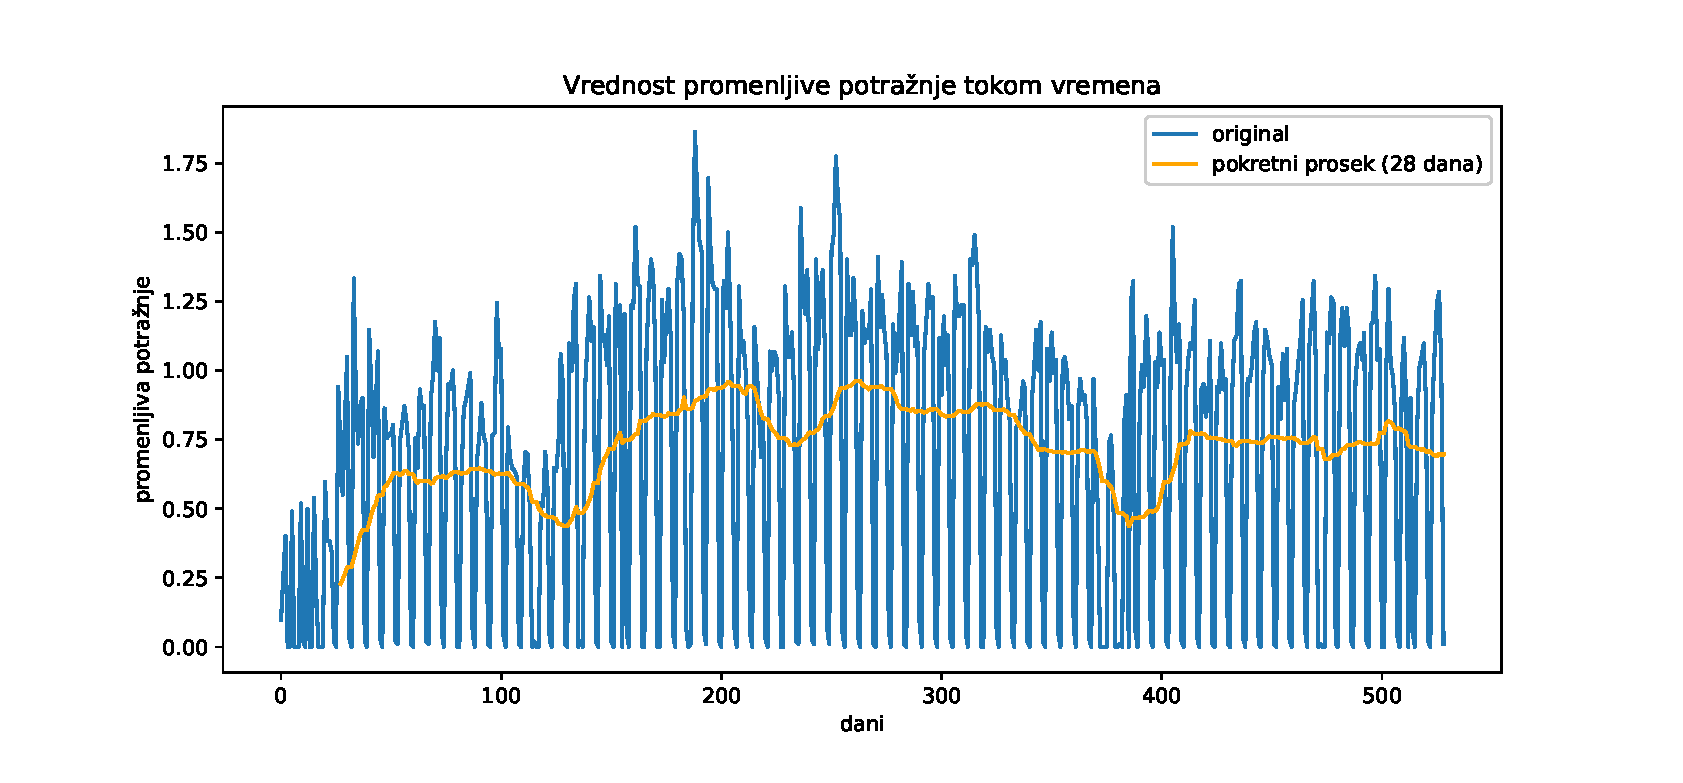
\includegraphics[width=1\textwidth]{./grafici/vremenska_serija_primer.eps}
  \caption{Primer vremenske serije iz rada}
  \label{fig:vremenska_serija}
\end{figure}

\subsection{Problem posmatran kroz atribute}
Kako razumevanje problema u vidu vremenske serije nije davalo značajne rezultate na većim granularnostima podataka, problem je posmatran kao regresioni problem koji zavisi od nekoliko atributa koji ga opisuju i rešavan je ansambl metodom ekstremnog gradijentnog pojačavanja. Cilj je bio pronaći vezu između dostupnih atributa i ciljne promenljive koja predstavlja vrednost potražnje. Primer skupa atributa i ciljne promenljive prikazan je na grafiku \ref{fig:atributi}, a opis metode rešavanja ovakvog problema biće predstavljen u sledećoj sekciji.

\begin{figure}[!ht]
  \centering
  \includegraphics[width=1\textwidth]{./grafici/atributi_primer.png}
  \caption{Primer skupa atributa i ciljne promenljive iz rada}    
  \label{fig:atributi}
\end{figure}

\section{Pregled dosadašnjih istraživanja}
Podaci korišćeni u radu dolaze iz novog izvora (pokrenut krajem 2019. godine), koji je dostupan korisnicima za rezervisanje popravki automobila, tako da su istraživanja nad ovim podacima prilično mlada i ne javno dostupna. Što se tiče same automobilske industrije i predviđanja potražnje vezane za popravke automobila i rezervne delove, takva istraživanja postoje. U radu \cite{faccio2010forecasting} na stranicama 18-22, dat je veoma detaljan pregled različitih metoda koje se koriste za predviđanja kao što su: Single Exponential Smoothing, Croston's Method, Moving Average, ARIMA, Neural Network... kao i detaljan tabelarni pregled autora koji su koristili neke od metoda u svojim istraživanjima. U master radu \cite{henkelmann2018deep}, prikazan je opširan pristup predviđanju potražnje automobilskih rezervnih delova dubokim učenjem. 

Rad \cite{zunic2020application} se bavi predviđanjem prodaje proizvoda u maloprodajnoj industriji nad realnim podacima, korišćenjem Prophet alata za predviđanje kod vremenskih serija. U radu \cite{saravanan2019forecasting} je predstavljeno predviđanje prodaje rezervnih delova ARIMA metodom. Navedeni pregled istraživanja potvrđuje koliko je problem predviđanja potražnje zastupljen u svakodnevnom svetu i pokazuje širinu isprobanih metoda koje mogu biti iskorišćene za rešavanje problema. Neke od navedenih metoda će biti isprobane u ovom radu.

% % Primer korišćenja tabele
% \begin{table}
% \centering
% \caption{Rezultati}
% \label{tbl:rezultati}
% \begin{tabular}{c>{\centering}p{2cm}c}
% \toprule
% 1 & 2 & 3\\\midrule
% 4 & 5 & 6\\\cmidrule(rl){1-2}
% 7 & 8 & 8\\
% \bottomrule
% \end{tabular}
% \end{table}

% % primer referisanja na poglavlja i strane poglavlja
% Više detalja biće dato u glavi \ref{chp:razrada} na strani \pageref{chp:razrada}.

% ------------------------------------------------------------------------------
\chapter{Opis korišćenih metoda i metrika}
\label{chp:metode}
U ovom poglavlju biće dat kratak pregled korišćenih metoda za rešavanje definisanog problema (videti poglavlje \ref{section:opis_problema}) predviđanja potražnje u industriji popravke automobila. Te metode su: 
\begin{enumerate}
    \item ARIMA
    \item Prophet
    \item XGBoost
\end{enumerate}
Pored korišćenih metoda, ukratko će biti opisane i metrike za evaluaciju modela i nekoliko pojmova značajnih za rad.

\section{ARIMA}
ARIMA (\textit{eng.} Autoregressive Integrated Moving Average) predstavlja algoritam za predviđanje ciljne promenljive kod vremenskih serija. Ona je dizajnirana da identifikuje obrasce u potražnji koja se desila i obrasce koji se ponavljaju kroz vreme \cite{mello2013demand}. Takođe, ARIMA je model univarijantne vremenske serije, gde je predviđanje zasnovano isključivo na prethodnim vrednostima. Ovaj metod objašnjava promene kroz tri komponente: (p, d, q). 

Prva komponenta - p, predstavlja autoregresivnu komponentu modela AR(p). Ona predstavlja vezu (linearnu regresiju) između trenutne vrednosti vremenske serije i njenih prethodnih p-vrednosti, sa parametrima koji predstavljaju težine uticaja prethodnih vrednosti na trenutnu vrednost. AR(p) se može predstaviti jednačinom \ref{eq: ar_p}, gde je $\epsilon_t$ šum/greška (\textit{eng.} white noise), $\phi$ su vrednosti AR parametara, $y_t$ je vrednost serije u vremenu t, $\mu$ je prosek promenljive y, p je vrednost kašnjenja.
\begin{equation}
\begin{gathered}
\label{eq: ar_p}
y_t = \delta + \phi_1y_{t-1} + \phi_2y_{t-2} + \dots + \phi_py_{t-p} + \epsilon_t \\
\delta = (1 - \phi_1 - \phi_2 - \dots - \phi_p)\mu \\
\end{gathered}
\end{equation}
Druga komponenta - d, predstavlja operaciju diferenciranja (I(d)) primenjenu d puta na vremensku seriju, sa ciljem da serija postane stacionarna \footnote{Vremenska serija je stacionarna kada sve njene vrednosti fituju istoj raspodeli verovatnoće, nevezano za vreme \cite{vargas2017automobile}. Odnosno, kada serija nema trend ili sezonske efekte i kad su statistička svojstva konstanta kroz vreme \cite{saravanan2019forecasting}.}. Diferenciranje (\textit{eng.} differencing) predstavlja pojam promene između 2 uzastopne posmatrane vrednosti u originalnoj seriji. Ono se može predstaviti jednačinom \ref{eq: diff}.
\begin{equation}
\label{eq: diff}
y'_t = y_t - y_{t-1}
\end{equation}
Treća komponenta - q, predstavlja komponentu klizajućih proseka (\textit{eng.} moving averages) i služi da objasni trenutnu $\epsilon_t$ vrednost tj. grešku, u odnosu na prethodnih q  vrednosti greške. MA(q) model se može predstaviti jednačinom \ref{eq: ma_q} \cite{vargas2017automobile}, gde $\theta$ vrednosti predstavljaju vrednosti MA parametara, q je vrednost kašnjenja.
\begin{equation}
\begin{gathered}
\label{eq: ma_q}
\tilde{y_t} = \epsilon_t - \theta_1\epsilon_{t-1} - \theta_2\epsilon_{t-2} - \dots - \theta_q\epsilon_{t-q}  \\
\tilde{y_t} = y_t - \mu
\end{gathered}
\end{equation}
Procesi mogu da imaju obe komponente: AR i MA. Kada se ukombinuju prethodne jednačine, finalni model je predstavljen jednačinom \ref{eq: arma}.
\begin{equation}
\label{eq: arma}
\tilde{y_t} - \phi_1\tilde{y_{t-1}} - \dots - \phi_p\tilde{y_{t-p}} = \epsilon_t - \theta_1\epsilon_{t-1} - \dots - \theta_q\epsilon_{t-q}
\end{equation}

ARIMA može da ima i sezonske komponente: (P, D, Q), kada se nazima SARIMA. Sezonske komponente predstavljaju regularne obrasce promena koje se ponavljaju svakih S vremenskih perioda, gde je S broj vremenskih perioda dok se obrazac opet ne ponovi. Detaljnije o SARIMA modelu se može naći u \cite{hyndman2018forecasting}.

\section{Prophet}
Prophet je alat za predviđanje ciljne promenljive kod vremenskih serija. Razvijen je od strane Facebook zajednice \cite{prophet} i može da generiše prognoze razumnog kvaliteta. Alat je otvorenog tipa (\textit{eng.} open-source) i zasnovan je na aditivnom modelu, gde se nelinearni trendovi fituju sa godišnjom, nedeljnom i dnevnom sezonalnošću (\textit{eng. seasonality}). Ono što Prophet ima kao opciju je uključivanje efekta praznika u model. Robustan je na nedostajuće vrednosti i promene u trendu, i tipično dobro obrađuje vrednosti van granica (\textit{eng.} outliers) \cite{zunic2020application}.

Originalni rad u kome autori predstavljaju Prophet \cite{taylor2018forecasting}, pomenuti model je predstavljen jednačinom \ref{eq: prophet}.
\begin{equation}
\label{eq: prophet}
y(t) = g(t) + s(t) + h(t) + \epsilon_t
\end{equation}
U jednačini \ref{eq: prophet}, g(t) predstavlja funkciju trenda koja modeluje neperiodične promene vrednosti ciljne promenljive, s(t) predstavlja periodične promene (npr. sezonske promene dnevnog ili godišnjeg nivoa), h(t) predstavlja efekat praznika koji mogu da se javljaju u neregularnim trenucima i da traju 1 ili više dana, $\epsilon_t$ se odnosi na grešku i obuhvata sve promene neuhvaćene modelom. Pretpostavka koju autori pominju u radu je da $\epsilon_t$ ima normalnu raspodelu. Pored navedenih opcija, moguće je kreirati sopstveni sezonski efekat (npr. mesečni) koji se generiše koristeći parcijalne Furijeove sum, kao i dosta drugih manuelnih opcija\footnote{Više se može pročitati na \url{https://facebook.github.io/prophet/}}. Prophet ima podršku za programski jezik Python i programski jezik R.

\section{XGBoost}
XGBoost (\textit{eng.} Extreme Gradient Boosting) je metod ekstremnog gradijentnog pojačavanja. Osnovna ideja metoda pojačavanja je da se ansambl izgradi dodavanjem jednog po jednog modela, gde svaki model uči tako da što bolje nadomesti mane trenutnog skupa modela. AdaBoost je prvi algoritam pojačavanja i radi po principu uvećavanja težina onih instanci koje su pogrešno klasifikovane, pa se sledeći model fokusira na te instance kako bi se celokupno stanje poboljšalo. 

Osim pojačavanja, postoje i gradijentna pojačavanja i ona su po pitanju preciznosti među najboljim metodama mašinskog učenja. Osnovna ideja ovih metoda dolazi iz gradijentnih optimizacionih problema, gde se tekuće rešenje popravlja dodavanjem vektora proporcionalnog negativnoj vrednosti gradijenta funkcije koja se minimizuje \cite{ml}. 

Ekstremno gradijentno pojačavanje predstavlja ansambl sistem pojačavanja zasnovan na drvetima odlučivanja. Evolucija algoritama je predstavljena na slici \ref{fig: xgboost_evolucija} i može se videti da je regularizacija jedna od novina kod XGBoost metode.

\begin{figure}[!ht]
  \centering
  \includegraphics[width=1\textwidth]{./grafici/xgboost_evolucija.png}
  \caption[Razvoj algoritama. Izvor: \textit{towardsdatascience}]
  {Razvoj algoritama. Izvor: https://towardsdatascience.com/https-medium-com-vishalmorde-xgboost-algorithm-long-she-may-rein-edd9f99be63d}
  \label{fig: xgboost_evolucija}
\end{figure}
Sam algoritam je poznat po svojoj skalabilnosti, dobrom ponašanju sa retkim (\textit{eng.} sparse) podacima, distribuiranosti i algoritam je podržan od strane nekoliko programskih jezika, među kojima je i Python \cite{chen2016xgboost}.

\section{Metrike}
Kroz rad je ispraćeno nekoliko metrika za evaluaciju modela. Korišćene metrike su:
\begin{itemize}
    \item Srednja apsolutna greška (MAE)
    \item Srednje kvadratna greška (MSE)
    \item Koren srednje kvadratne greške (RMSE)
    \item Simetrična srednja apsolutna procentualna greška (SMAPE)
\end{itemize}
Ključna metrika koja je praćena je SMAPE, ali i ostale metrike su propraćene kroz modele. U nastavku će biti detaljnije opisana SMAPE metrika.

\subsection{SMAPE}
SMAPE (\textit{eng.} Symmetric Mean Average Percentage Error) metrika je izmenjena za potrebe projekta i formula po kojoj je računata je predstavljena jednačinom \ref{eq: smape}.
\begin{equation}
\label{eq: smape}
SMAPE = \frac{\sum\limits_{t=1}^{N} |F_t - A_t|} {\sum\limits_{t=1}^{N}max(A_t, F_t)}
\end{equation}
U formuli $F_t$ predstavlja prediktovanu vrednost u vremenu t, $A_t$ predstavlja stvarnu vrednost u vremenu t, a N je broj instanci. Manje vrednosti ove metrike su pogodnije za predikcije i u praksi se pokazalo da modeli sa vrednostima manjim od 0.3 imaju nekog smisla.
\newline
\\
Osim metrika za evaluaciju modela, korišćena je Akaike Information Criterion\footnote{\url{https://en.wikipedia.org/wiki/Akaike_information_criterion}} (AIC) metrika za evaluaciju ARIMA modela kod vremenskih serija. Ona je računata ugrađenom funkcijom u programskom jeziku Python. Manja vrednost ove metrike označava bolji model.

\section{Impact Encoding}
\label{lbl: impact_encoding}
Impact Encoding predstavlja jednu vrstu enkodiranja kategoričkih atributa u redne vrednosti. Ono predstavlja nadogradnju na Target Encoding \cite{pargent2019benchmark} i praktičnije je od one-hot enkodiranja zbog toga što dodaje samo 1 kolonu koja predstavlja izlaz, za razliku od one-hot enkodiranja. Sastoji se od 3 koraka: Target Encoding, regularizacija i normalizacija.

Target Encoding je deo koji svaku vrednost kategoričkog atributa zamenjuje prosečnom vrednošću koju baš ta vrednost kategoričkog atributa ima u koloni ciljne promenljive. Recimo, ako je kategorički atribut boja i ona može da uzme vrednosti: crvena i plava, onda crvenu enkodiramo sa prosekom vrednosti koju crvena ima u koloni ciljne promenljive. Ovo se može zapisati sledećom formulom u kojoj T predstavlja vrednost kategoričkog atributa $c_v$ u koloni ciljne promenljive: 

\begin{center}
$c_v \to \frac{\sum{T_{c_v}}}{|c_v|}$ 
\end{center}
Deo regularizacije enkodiranja se bavi problemom da ne verujemo baš svakom mapiranju vrednosti jednako. Ovaj problem se javlja u praksi kada vrednost ciljne promenljive za jednu vrednost kategoričkog atributa može da bude ogromna, a da te vrednosti atributa ima jako malo; naspram puno vrednosti kategoričkog atributa čije su vrednosti koje odgovaraju ciljnoj promenljivoj dosta manje. Želimo da izbalansiramo ovu situaciju i to se rešava uvođenjem parametra $\alpha := \max |c_v|$, koji predstavlja maksimum broja pojavljivanja vrednosti kategoričkog atributa. Tada enkodiranje postanje mapiranje atributa u: 

\begin{center}
$c_v \to \frac{|c_v|\mu_{c_v} + \alpha\mu_c}{|c_v| + \alpha}$
\end{center}
Deo normalizacije rešava problem kada Impact Encoding radimo nad trening podacima, a u test skup nam dođe vrednost atributa koja nije viđena u trening skupu dok smo vršili mapiranje vrednosti. Rešenje u ovoj situaciji je normiranje sa prosekom svih klasa:
\begin{center}
$c_v \to \frac{\frac{|c_v|\mu_{c_v} + \alpha\mu_c}{|c_v| + \alpha}}{\mu_{c}}$
\end{center}
Ovako nepoznatim instancama može da se dodeli vrednost 1, koja implicira da je impact očekivana srednja vrednost svih klasa i da nema odstupanja od populacije.

% ------------------------------------------------------------------------------

% ------------------------------------------------------------------------------
\chapter{Prikaz rada metoda i rezultati}

\section{Podaci}
Podaci korišćeni u radu su prikupljeni od jedne Švedske kompanije. Predstavljaju realne podatke iz industrije, a važno je napomenuti da su dobijeni sa samo jednog izvora koji je dostupan njihovim korisnicima. Radi se o novom načinu rezervisanja popravki automobila na različitim lokacijama, putem interneta (\textit{eng.} booking portal). Portal je krenuo sa radom krajem 2019. godine, tako da je količina podataka ograničena. Takođe, 2020. godina je bila udarna godina virusa Covid19 \cite{madabhavi2020covid}, tako da ograničena količina dostupnih podataka i istraživanje nad njima možda bude od posebnog značaja u budućnosti, pre svega kada pomenuti booking portal bude izvor veće količine informacija.

Podaci se sastoje od informacija kao što su: koja marka automobila je došla u koju registrovanu automehaničarsku radnju, kog datuma i od nekih informacija vezanih za popravku. Svi korišćeni kategorički atributi su morali biti zamaskirani i kodirani kombinacijama slova zbog privatnosti firme, a svi numerički atributi su normirani. Na slici \ref{fig:atributi} se može videti primer korišćenog skupa podataka za predviđanje promenljive \textit{demand\_value}, na granularnosti marki automobila i  automehaničarskih radnji, na nivou nedelja. Atributi \textit{x\_units} i \textit{x\_unit\_cost} su vezani za informacije o konkretnim rezervacijama, od kojih u modelima nije korišćen \textit{x\_units}, kako ne bi dolazilo do potencijalnog curenja informacija u modelu.

\subsection{Obogaćivanje podataka eksternim podacima}
Atributi \textit{number\_of\_competitors} i \textit{reachable\_population} su generisani na osnovu firminih informacija o lokacijama automehaničarskih radnji. Za svaku radnju su poznate geografska širina i geografska dužina. Atribut \textit{reachable\_population} je kreiran od strane zaposlenih u firmi, na osnovu javnih statističkih podataka o populaciji stanovništva u regionima radnji. On predstavlja sumu populacije velikih regiona u radijusu koji predstavlja distancu pređenu za 40 minuta vožnje, brzinom 60 km/h, od lokacije radnje. 

Atribut \textit{number\_of\_competitors} je dodat u sklopu ovog rada. On predstavlja broj drugih radnji (konkurenata) u radijusu od 80km od automehaničarske radnje. Vrednost od 80km je uzeta kao neka racionalna vrednost za voženje do neke recimo jeftinije radnje ili do radnje koja nije u drugom gradu. Vrednost ovog atributa je kreirana korišćenjem Open Street Map (OSM)\footnote{\url{https://www.openstreetmap.org}}, odnosno besplatne mape sveta. OSM ima besplatan servis za dohvatanje raznih informacija na osnovu zadatih parametara, korišćenjem njihovog upitnog jezika. Servis se zove Overpass API\footnote{\url{https://overpass-turbo.eu}} i zadavanjem lokacija radnji i specijalnog taga \textbf{\textit{'shop'='car\_repair'}} dobijene su informacije o radnjama u okolini u \textit{json} formatu. Primer koda korišćen za dohvatanje informacija o radnjama je prikazan u listingu \ref{lbl: overpass_funkcija}.\\
\begin{lstlisting}[language=python, belowskip=-\baselineskip, frame=single, label=lbl: overpass_funkcija, caption={Funkcija za dohvatanje informacija o drugim radnjama u okolini.}]
overpass_url = "http://overpass-api.de/api/interpreter"

def overpass_query(latitude, longitude, km_around):
    overpass_query = "[out:json];(node(around:{},{},{})['shop'='car_repair'];);out;".format(km_around, latitude, longitude)

    while True:
        try:
            response = requests.get(overpass_url, params={'data': overpass_query})
            garages_around = response.json()
            return garages_around
        except:
            print("Try again...")
\end{lstlisting} 
\vspace{20pt}
Primer informacija koje se dobiju upitom ka Overpass API prikazan je na slici \ref{fig: overpass}. Za atribut skupa podataka u ovom radu, korišćen je samo ukupan broj radnji u okolini. 

\begin{figure}[!ht]
  \centering
  \includegraphics[width=1\textwidth]{./grafici/overpass_primer.png}
  \caption{Overpass API primer upita.}
  \label{fig: overpass}
\end{figure}

Primer podataka koji je korišćen za vremenske serije na dnevnom nivou predstavljen je na slici \ref{fig: daily_data_example}, a na nedeljnom nivou na slici \ref{weekly_data_example}. Bitno je napomenuti da su datumi prebačeni u nedelje u godini, tako da se vodilo računa o tome da kalendarski dan bude u tekućoj kalendarskoj godini, npr. da 30. decembar 2019. godine bude u poslednjoj nedelji 2019. godine, a ne u prvoj nedelji 2020. godine. Odluka da tako bude je napravljena u dogovoru sa firmom, da bude usaglašena sa kalendarskom godinom i kalkulacijama na nivou godine. Primer koda koji sređuje prebacivanje, kao i izvor sa svim podacima korišćenim u radu, dat je u Github repozitorijumu projekta, na adresi: \url{https://github.com/mandja96/matf-master-rad}.

\begin{figure}[!ht]
  \centering
  \includegraphics[width=0.4\textwidth]{./grafici/daily_data_example.png}
  \caption{Primer korišćenih podataka za dnevnu vremensku seriju.}
  \label{fig: daily_data_example}
\end{figure}

\begin{figure}[!ht]
  \centering
  \includegraphics[width=0.4\textwidth]{./grafici/weekly_data_example.png}
  \caption{Primer korišćenih podataka za nedeljnu vremensku seriju.}
  \label{fig: weekly_data_example}
\end{figure}

\section{Dnevni nivo - na nivou države} 
U ovom poglavlju biće predstavljeni propraćeni koraci i dobijeni rezultati nad dnevnim podacima, koji predstavljaju univarijantnu vremensku seriju. Podaci su agregirani po datumima, za nivo cele države. Biće izložena tri pristupa: Arima, Prophet i XGBoost, koji su opisani u poglavlju \ref{chp:metode}. Razlog posmatranja vremenske serije nad agregiranim podacima je pre svega da se isproba ponašanje metoda, ali i da se upoznaju podaci i generalni nedostatak podataka za vremensku seriju nad zasebnim radnjama i markama (većim granularnostima-manjoj agregaciji). 

\subsubsection{Pretprocesiranje dnevnih podataka}
Pre svega je ispitano koliko datuma nedostaje u vremenskoj seriji u vremenskom periodu 18. decembar 2019 - 29. maj 2021. Broj nedostajućih dana je 96 i ti dani su popunjeni vrednošću 0. Odnos nula i ne-nula dana prikazan je na histogramu \ref{fig: nula_nenula}, a raspodela nedostajućih dana po danima nedelje je prikazana na histogramu \ref{fig: dani_nedelje}. 

\begin{figure}[!ht]
  \centering
  \includegraphics[width=1\textwidth]{./grafici/nula_vrednosti_dnevni_podaci.eps}
  \caption{Procenat pozitivnih i nula vrednosti promenljive potražnje, nakon popunjavanja nedostajućih datuma.}
  \label{fig: nula_nenula}
\end{figure}

\begin{figure}[!ht]
  \centering
  \includegraphics[width=1\textwidth]{./grafici/nule_po_danima_nedelje.eps}
  \caption{Raspodela nula vrednosti promenljive potražnje po danima u nedelji.}
  \label{fig: dani_nedelje}
\end{figure}

Kao što se može videti sa histograma, većina 0 vrednosti pripada nedeljama. Ostatak datuma koji imaju vrednost nula su pretežno neki praznici koji su neradni dani (oko Nove godine, Uskrsa, državnog praznika...). Zbog velike zastupljenosti 0 vrednosti kod nedelje kao dana u sedmici, sve nedelje su izbačene iz vremenske serije i serija je posmatrana kao da postoji 6 dana u sedmici. Veličina posmatranih dana je nakon toga postala 454.

\subsection{Arima}
Kod Arime je bilo bitno ispitati neka svojstva vremenske serije kao što su nedostajuće vrednosti (datumi), stacionarnost, sezonski efekti. Takođe, bilo je bitno ispitati ACF i PACF plotove, kako bi se odredili parametri (p, d, q) koji konstruišu model, ali ispitati i kako se ponaša sezonska Arima (SARIMA) nad podacima.

Nakon pomenutog pretprocesiranja podataka, vremenska serija ima izgled prikazan na grafiku \ref{fig: dnevna_vremenska_serija_bez_nedelja}. 

\begin{figure}[!ht]
  \centering
  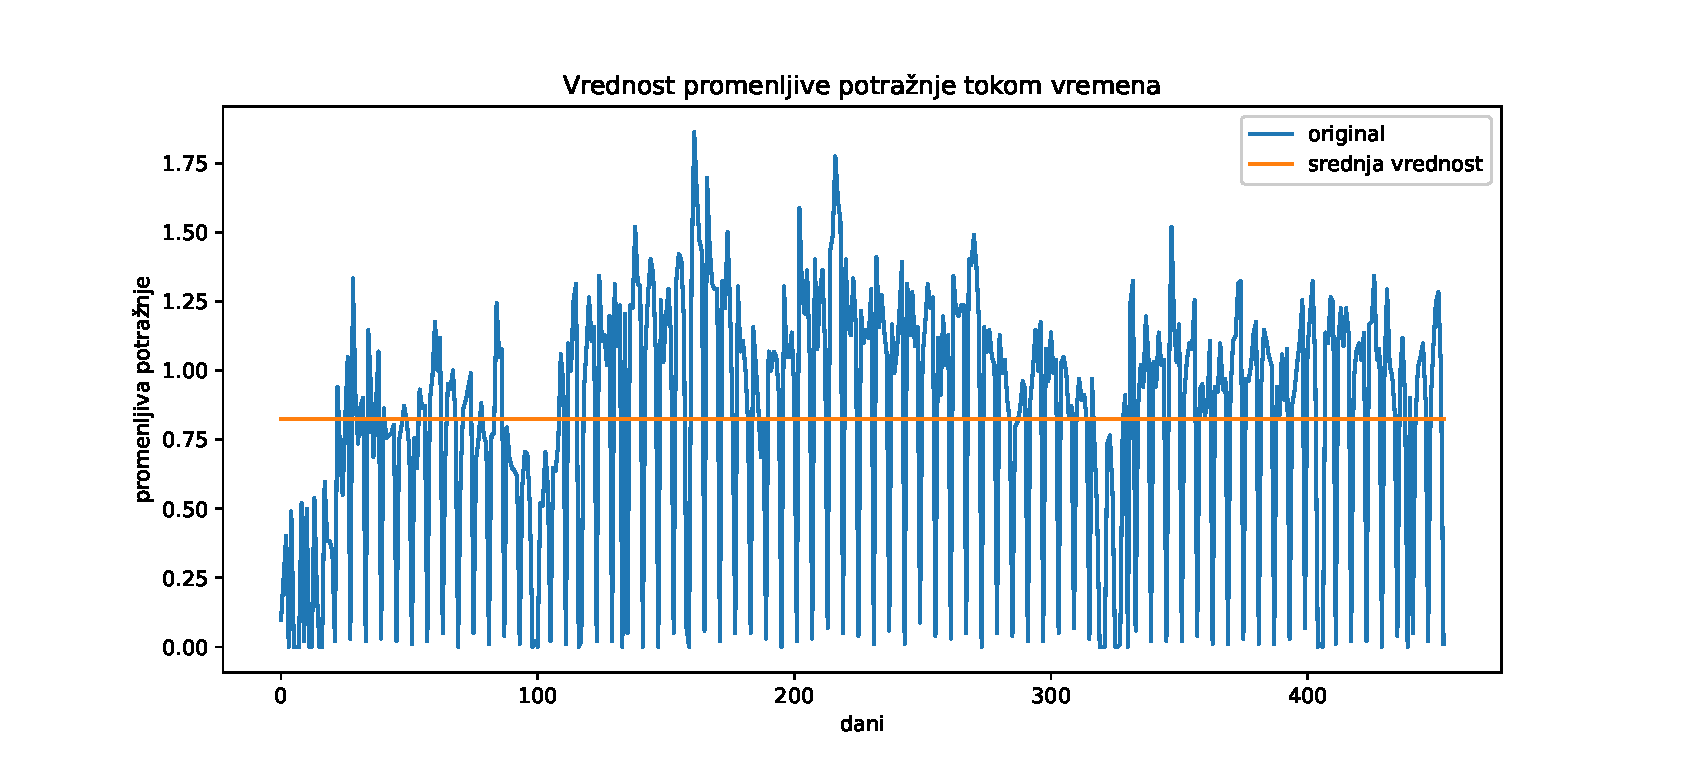
\includegraphics[width=1\textwidth]{./grafici/vremenska_serija_primer_bez_nedelja.eps}
  \caption{Vremenska serija bez nedelja.}
  \label{fig: dnevna_vremenska_serija_bez_nedelja}
\end{figure}

Prva sledeća stvar je bila ispitivanje stacionarnosti serije, jer je na osnovu toga doneta odluka da li seriju treba diferencirati ili ne. U ove svrhe korišćen je statistički \textbf{Augmented Dickey-Fuller} test. Ovaj test se može pronaći implementiran u paketu \textit{statsmodels} pod nazivom \textbf{\textit{adfuller}}. Vrednost testa nad dnevnim podacima bez nedelja je vratila vrednosti:
\begin{verbatim}
Test Statistics                 -3.674781
p-value                          0.004482
No. of lags used                18.000000
Number of observations used    435.000000
critical value (1%)             -3.445473
critical value (5%)             -2.868207
critical value (10%)            -2.570321
\end{verbatim}
Odavde se može zaključiti da je p-vrednost manja od 0.05 i da se nulta hipoteza može odbaciti, što nam govori da je serija stacionarna i da nema potrebe za diferenciranjem. Dakle, parametar d=0. Takođe, radi dodatne provere, iz paketa \textbf{pmdarima} iskorišćena je ugrađena funkcija \textit{ndiffs}, koja vraća vrednost parametra d (u ovom slučaju 0).

Sledeće je potrebno ispitati koje vrednosti parametri p i q mogu potencijalno da imaju. Za ispitivanje ovih parametara nam mogu pomoći ACF i PACF plotovi. Na grafiku \ref{fig: acf_pacf_dnevni} se mogu videti plotovi za ove podatke. Primećujemo da originalni podaci imaju pikove na svakih 6 stubića. To nam govori da postoji možda neka sezonalnost, tako da su propraćeni i ACF/PACF plotovi sa razlikom trenutne vrednosti i vrednosti u trenutku 6 vrednosti u prošlosti. Za dobijanje ovih grafika korišćene su funkcije \textbf{plot\_acf} i \textbf{plot\_pacf} iz paketa \textit{statsmodels}.

\begin{figure}[!ht]
  \centering
  \includegraphics[width=1\textwidth]{./grafici/acf_pacf_dnevni.png}
  \caption{ACF i PACF grafici. Na x-osi su lagovi, a na y-osi vrednost korelacije.}
  \label{fig: acf_pacf_dnevni}
\end{figure}
Na osnovu knjige \cite{hyndman2018forecasting}, sa plotova se može zaključiti da se radi o ARIMA(0, 0, 0)(0, 0, 1)[6] modelu. To je sezonska Arima (SARIMA) koja ima MA=1, ali sa kašljenjem od 6 dana. Dakle, ovo sugeriše da za predviđanje ponedeljka treba gledati u vrednosti prethodnog ponedeljka, za predviđanje utorka vrednosti prethodnog utorka itd, jer je na vrednosti 6 kod ACF plota najviši stubić.

Pokretanjem \textbf{auto\_arima} funkcije iz paketa \textit{pmdarima}, najbolji model je ARIMA(2, 0, 0)(2, 0, 1)[6]. On je dobijen gledanjem u minimalnu vrednost AIC metrike opisane u poglavlju \ref{chp:metode}. Kako su dva SARIMA modela sugerisala da treba gledati u jednu ili 2 vrednosti 6 dana u prošlosti, ispitan je i model ARIMA(6, 0, 6) i model ARIMA(9, 0, 6) koji je dobijen \textbf{auto\_arima} funkcijom kada se isključi sezonski parametar. Pored njih, iz radoznalosti, ispitani su i modeli ARIMA(1, 0, 1), ARIMA(1, 0, 0), ARIMA(1, 0, 1)(1, 0, [1,2])[6]. Vrednosti AIC metrike su prikazane u tabeli \ref{tbl: arime_aic}, vrednosti metrika evaluacije u tabeli \ref{tbl: arime_metrike}, a autokorelacioni grafik reziduala najboljeg modela na slici \ref{fig: reziduali} (dobijen je funkcijom \textit{plot\_diagnostics} nad modelom ARIMA(1, 0, 1)(1, 0, [1, 2])[6]). Reziduali treba da nemaju korelaciju, kako bi predstavljali samo šum (\textit{eng.} white noise).

\begin{table}
\centering
\caption{SARIMA/ARIMA vrednosti AIC metrike}
\label{tbl: arime_aic}
\begin{tabular}{ |l|c| } 
\hline
model & AIC \\
\hline
ARIMA(1, 0, 1) & 567.39\\ 
ARIMA(1, 0, 0) & 598.30\\ 
ARIMA(6, 0, 6) & 14.31\\ 
ARIMA(9, 0, 6) & 14.63\\
ARIMA(1, 0, 1)(1, 0, [1,2])[6] & 3.81\\
ARIMA(2, 0, 0)(2, 0, 1)[6] & 8.57\\
\hline
\end{tabular}
\end{table}

\begin{table}
\centering
\caption{SARIMA/ARIMA metrike evaluacije}
\label{tbl: arime_metrike}
\begin{tabular}{ |l|c|c|c|c|} 
\hline
model & mae & mse & rmse & smape \\
\hline
ARIMA(1, 0, 1) & 0.389531 & 0.230040 & 0.479625 & 0.379000 \\ 
ARIMA(1, 0, 0) & 0.382899 & 0.215804 & 0.464547 & 0.375804\\ 
ARIMA(6, 0, 6) & 0.563536 & 0.094383 & 0.307218 & 0.213063\\ 
ARIMA(9, 0, 6) & 0.209452 & 0.095371 & 0.308821 & 0.224278\\ 
ARIMA(1, 0, 1)(1, 0, [1,2])[6] & 0.192394 & 0.094991 & 0.308206 & 0.208225\\
ARIMA(2, 0, 0)(2, 0, 1)[6] & 0.200078 & 0.092266 & 0.303753 & 0.215694\\
\hline
\end{tabular}
\end{table}

\begin{figure}[!ht]
  \centering
  \includegraphics[width=1\textwidth]{./grafici/reziduali_arima.png}
  \caption{Provera normalnosti i odsustva korelacije među rezidualima modela.}
  \label{fig: reziduali}
\end{figure}
Detaljan način obučavanja ARIME se može pronaći u kodovima na github repozitorijumu projekta. Princip obučavanja je bio da se u trening skupu na početku nalaze svi dani pre 1. marta 2021. godine, a da se zatim predviđa 1 po 1 dan u budućnost, nakon čega se u trening skup dodaje 1 dan. Modeli su evaluirani na osnovu predviđanja jednog dana u napred od 1. marta 2021. godine, treniranjem nad svim podacima pre. Takođe, predikcije su vršene i po nekoliko dana unapred odjednom (konkretno 28 dana), da se vidi ponašanje modela. Na grafiku \ref{fig: test_arima} se može videti ponašanje dva modela.
\begin{figure}[!ht]
  \centering
  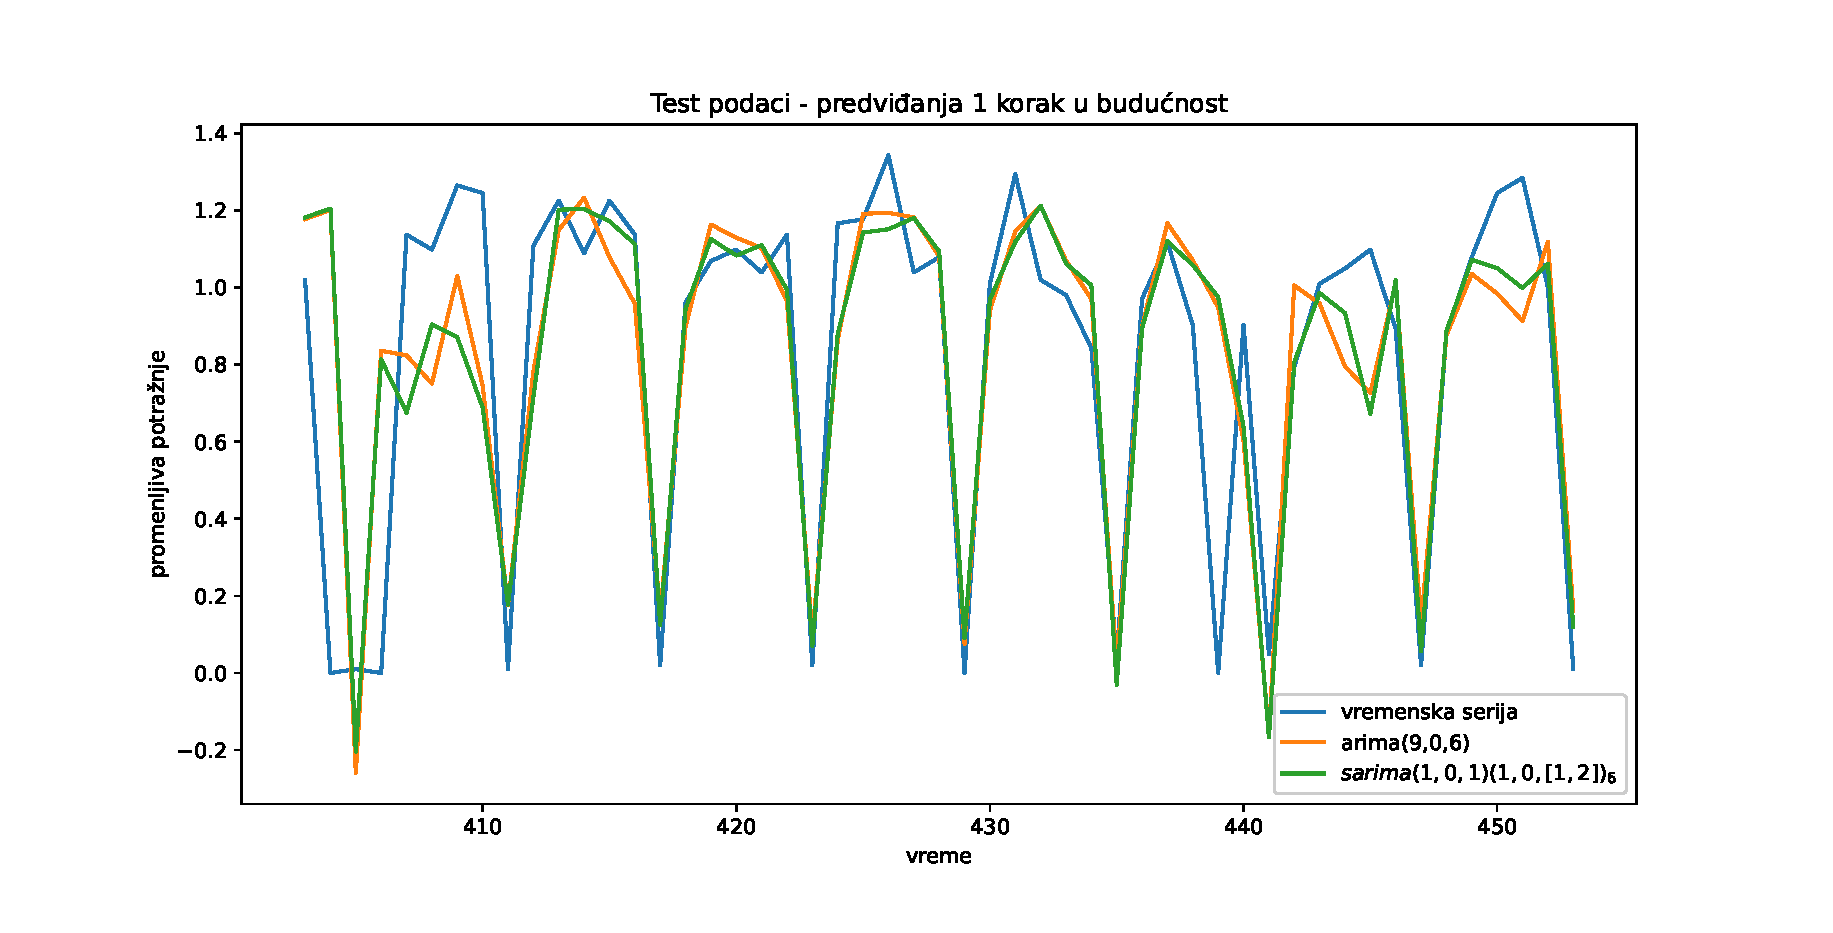
\includegraphics[width=1\textwidth]{./grafici/test_dnevna_arima.eps}
  \caption{Ponašanje 1 po 1 predviđanja dva modela kod arima metode.}
  \label{fig: test_arima}
\end{figure}

\subsection{Prophet}
Nad istim podacima i na isti način, isproban je i Facebook-ov alat Prophet. Puštena su 4 modela, sa uključenim praznicima u Švedskoj, pošto je to omogućena opcija kod ovog metoda.

Metrike za evaluaciju modela su prikazane u tabeli \ref{tbl: prophet_dnevni}, a grafik predviđanja na slici \ref{fig: test_prophet}. Sa grafika se može videti kako postoji jedan značajniji pad. Razlog tome je uračunavanje efekta praznika u modele, što je potvrdilo ideju da potencijalno treba uzimati u obzir praznike i u drugim modelima, ako je to moguće.
\begin{table}
\centering
\caption{Prophet metrike evaluacije}
\label{tbl: prophet_dnevni}
\begin{tabular}{ |l|c|c|c|c|} 
\hline
model & mae & mse & rmse & smape \\
\hline
prophet (w, m, h) & 0.120943 & 0.038284 & 0.195662 & 0.141016 \\ 
prophet (w, m, h, flexible) & 0.113431 & 0.032307 & 0.179741 & 0.129801\\
prophet (d, w, m, h) & 0.119556 & 0.035445 & 0.188267 & 0.139296 \\
prophet (d, w, m, h, flexible) & 0.113918 & 0.032443 & 0.180120 & 0.130383\\
\hline
\end{tabular}
\end{table}

\begin{figure}[!ht]
  \centering
  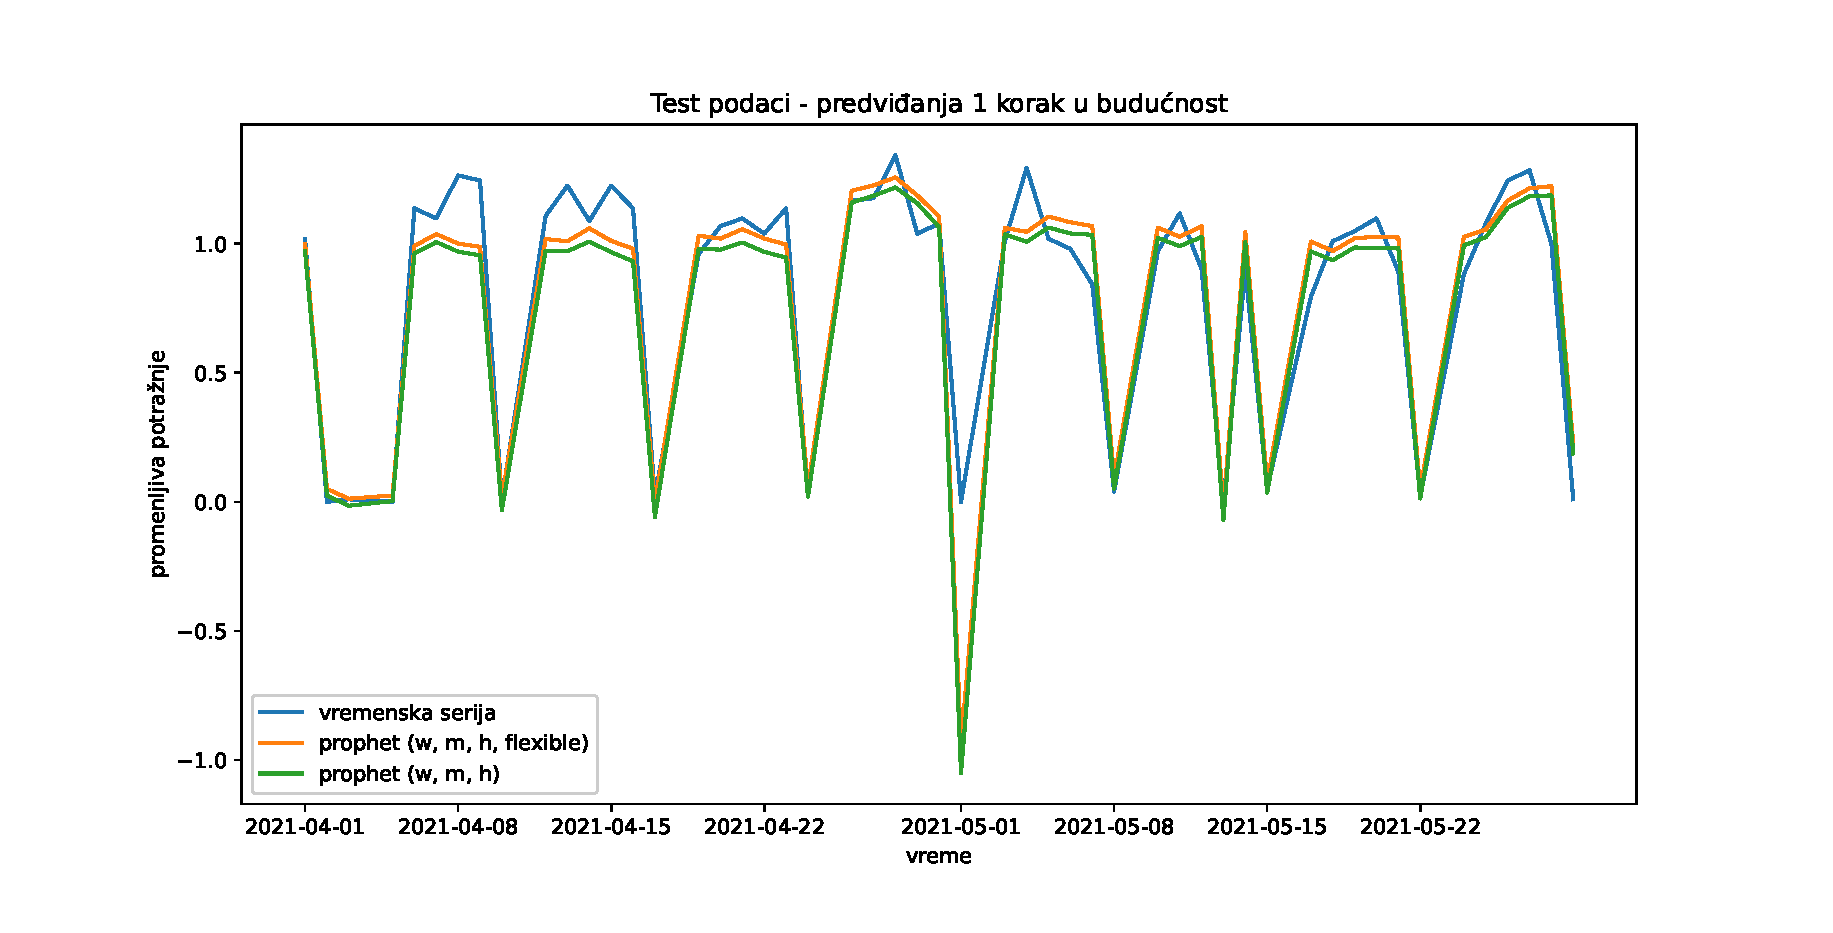
\includegraphics[width=1\textwidth]{./grafici/test_dnevni_prophet.eps}
  \caption{Ponašanje 1 po 1 predviđanja dva modela kod prophet metode. Razlog zašto test podaci počinju tek 1. aprila, a ne 1. marta, je zbog toga što je testirano predviđanje do 28 dana u napred, tako da konkateniranje skupova izbacuje nedostajuće vrednosti koje postoje 28 dana nakon 1. marta.}
  \label{fig: test_prophet}
\end{figure}
U tabeli su oznake koje predstavljaju informaciju da li su u model uključeni sezonski efekti i praznici. Oznake su: w - uključen nedeljni sezonski efekat, m - uključen mesečni sezonski efekat, h - uključeni praznici, d - uključen dnevni sezonski efekat i flexible označava postavljanje parametra \textit{changepoint\_prior\_scale}=0.09, što znači postavljanje trenda da bude više fleksibilan \footnote{\url{https://facebook.github.io/prophet/docs/trend_changepoints.html}}. 

\subsection{XGBoost}
XGBoost je isproban nad istim podacima, ali je sa njim urađen jedan eksperiment. Atributi za XGBoost nad dnevnim podacima su zapravo vrednosti promenljive potražnje (\textit{eng.} demand\_value) iz prethodnih nekoliko dana u prošlosti. Testirano je kako XGBoost radi sa 30 vrednosti iz prošlosti, sa tri dodata atributa koja predstavljaju praznike u Švedskoj. Praznici u Švedskoj su uzeti iz paketa \textit{holidays}, i 3 atributa predstavljaju: 
\begin{itemize}
    \item \textit{number\_of\_holidays\_next\_day} - broj praznika sledećeg dana
    \item \textit{number\_of\_holidays\_previous\_day} - broj praznika prethodnog dana
    \item \textit{number\_of\_holidays} - broj praznika u tekućem dana
\end{itemize}
Validacioni set za XGBoost je predstavljao 20\% test podataka koji kreću od 1. marta 2021. godine i korišćen je parametar \textit{early\_stopping\_rounds}=30, kako bi se sprečilo preprilagođavanje. Metrike evaluacije za ovako dobijeni model su predstavljene u tabeli \ref{tbl: xgboost_1}. 
\begin{table}
\centering
\caption{XGBoost metrike evaluacije}
\label{tbl: xgboost_1}
\begin{tabular}{ |l|c|c|c|c|} 
\hline
mae & mse & rmse & smape \\
\hline
0.112533 & 0.033992 & 0.184370 & 0.127315 \\ 
\hline
\end{tabular}
\end{table}
Važnost atributa (\textit{eng.} feature importance) ovakvog modela je predstavljena ispod:
\begin{verbatim}
    [0.00794075, 0.00629401, 0.00511439, 0.00234501, 0.00245581,
     0.42707652, 0.0020948 , 0.00207992, 0.00157057, 0.0035512 ,
     0.00304402, 0.00182108, 0.00567753, 0.00143691, 0.00109723,
     0.00155572, 0.0033229 , 0.08218686, 0.00293316, 0.00355283,
     0.00354679, 0.00391645, 0.00104043, 0.01375661, 0.0011694 ,
     0.00137136, 0.00357201, 0.00281513, 0.00125128, 0.00372967,
     0.39017874, 0.0065008 , 0.        ]
\end{verbatim}
Odavde se može zaključiti da XGBoost najveću vrednost daje vrednosti ciljne promenljive iz prethodnih 6 dana, iz prethodnih 18 dana i vrednosti broja praznika tekućeg dana.

Pored ovog eksperimenta, urađena su još 2 eksperimenta. Prvi je bio dodavanje na postojeće atribute još jedan atribut koji predstavlja prosek vrednosti prethodnih 6 dana. Drugi eksperiment je na prvobitne atribute dodao prosek razlike od srednje vrednosti za prethodnih 6 dana (pokušavajući da se imitira model arime sa MA=6 koeficijentom). Ovi eksperimenti su bili bezuspešni, sa atributima koji nisu doprineli poboljšanju modela. Na SHAP grafiku \ref{fig: shap_xgboost} se može videti kako 6. dan iz prošlosti doprinosi smanjenju vrednosti, a broj praznika u danu povećanju vrednosti ciljne promenljive. Ova analiza je urađena samo na celom trening setu osnovnog modela za koji su izložene metrike, kako bi se ispitalo ponašanje.
\begin{figure}[!ht]
  \centering
  \includegraphics[width=1\textwidth]{./grafici/shap_xgboost_dnevni.png}
  \caption{SHAP vrednosti nad trening skupom.}
  \label{fig: shap_xgboost}
\end{figure}

\section{Nedeljni nivo - na nivou države}
Primer podataka agregiranih na nedeljnom nivou, može se videti na slici \ref{fig: weekly_data_example}. Ta vremenska serija je predstavljena na grafiku \ref{fig: nedeljna_serija}. Ukupan broj dostupnih nedelja je 76. Prvo što se može primetiti kod ove vremenske serije su 2 veća pada vrednosti. Jedan se desio oko Uskrsa 2020. godine, a drugi se desio oko Nove godine.
\begin{figure}[!ht]
  \centering
  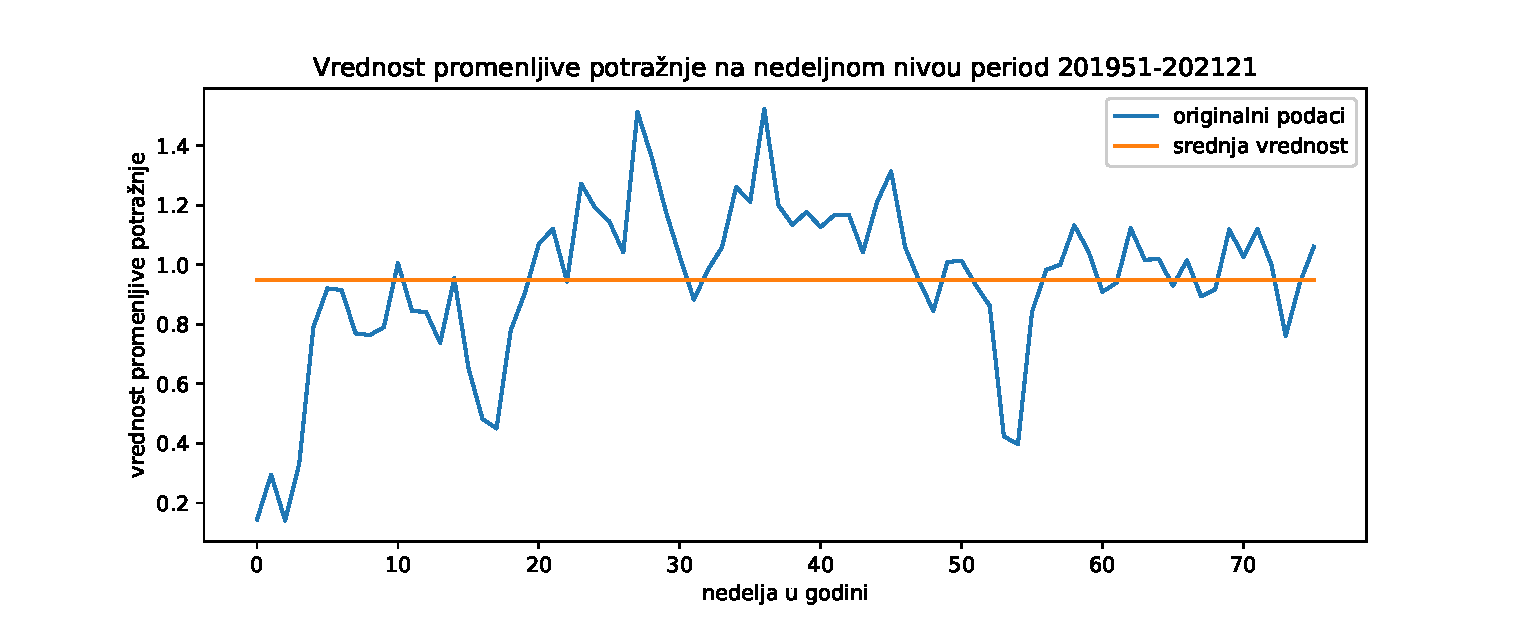
\includegraphics[width=1\textwidth]{./grafici/nedeljna_vremenska_serija.eps}
  \caption{Nedeljna vremenska serija.}
  \label{fig: nedeljna_serija}
\end{figure}
\subsection{Arima i Prophet}
Kao i kod primera nad dnevnim podacima, prva ispitivana stvar je stacionarnost vremenske serije. Statistički\textbf{Augmented Dickey-Fuller} test je korišćen i vrednosti rezultata nad nedeljnim podacima su sledeći:
\begin{verbatim}
Test Statistics                -3.915460
p-value                         0.001924
No. of lags used                0.000000
Number of observations used    75.000000
critical value (1%)            -3.520713
critical value (5%)            -2.900925
critical value (10%)           -2.587781
\end{verbatim}
    Može se zaključiti da je serija stacionarna i da bi vrednost parametra d trebala da bude 0, tj. da nema potrebe za diferenciranjem podataka. Kako se radi o nedeljnim podacima, za svaku nedelju neki podaci su sigurno dostupni, tako da ne postoje nedostajuće nedelje. Na grafiku \ref{fig: acf_pacf_nedeljni} su prikazani grafici ACF i PACF, sa ciljem da se bolje razume ponašanje serije i da se odrede najpogodnije vrednosti parametara p i q. Sa grafika vremenske serije se može zaključiti da nema nekih lako uočljivih sezonskih efekata, za dostupnu količinu podataka, a to potvrđuju i ACF/PACF plotovi. 
\begin{figure}[!ht]
  \centering
  \includegraphics[width=1\textwidth]{./grafici/acf_pacf_nedeljni.png}
  \caption{ACF i PACF grafici. Na x-osi su lagovi, a na y-osi vrednost korelacije.}
  \label{fig: acf_pacf_nedeljni}
\end{figure}
Ono što se praćenjem literature može zaključiti je da se radi o modelu ARIMA(1, 0, 2) najverovatnije. Stubića izvan značajne zone na PACF plotu, do prvog sledećeg stubića unutar zone, ima 1 što određuje AR parametar. Na grafiku ACF se nalaze 2 stubića izvan značajne zone, tako da nam je to neki indikator da je parametar MA=2. Model koji je funkcija \textbf{auto\_arima} vratila kao najbolji prema AIC metrici je ARIMA(1, 0, 0), dakle čist autoregresivni model koji predikcije pravi isključivo na jednoj prethodnoj vrednosti cilje promenljive. Pored ovih modela isprobani modeli su i: ARIMA(1, 1, 1), ARIMA(12, 1, 0) i ARIMA(13, 0, 2). Za model ARIMA(13, 0, 2) razlog je što PACF pokazuje značajan stubić na vrednosti kašnjenja (laga) 13, a ostali su isprobani iz radoznalosti. Rezultati AIC metrika za ARIMA modele su prikazani u tabeli \ref{tbl: arima_aic_nedeljna}.
\begin{table}
\centering
\caption{AIC metrika za ARIMA modele nad nedeljnim podacima.}
\label{tbl: arima_aic_nedeljna}
\begin{tabular}{ |l|c|} 
\hline
model & AIC \\
\hline
ARIMA(1, 0, 0) & -45.56447485932554\\
ARIMA(1, 1, 1) & -43.27962567290584\\
ARIMA(1, 0, 2) & -41.93537038126968\\
ARIMA(12, 1, 0) & -39.918282940344085\\
ARIMA(13, 0, 2) & -35.86521951018952\\
\hline
\end{tabular}
\end{table}
Iz priložene tabele (\ref{tbl: arima_aic_nedeljna}) se može primetiti da postoji bolji model po AIC vrednosti od modela koji je funkcija iz \textit{statsmodels} paketa predložila. Na test podacima su evaluirane metrike i ta statistika je prikazana u tabeli \ref{tbl: nedeljna_serija_metrike}. Pored ARIMA metoda, isprobana su i dva Prophet modela, koja su se istraživanjem pokazala kao najbolja. 
\begin{table}
\centering
\caption{Evaluacione metrike nad test podacima nedeljne vremenske serije.}
\label{tbl: nedeljna_serija_metrike}
\begin{tabular}{ |l|c|c|c|c|} 
\hline
model & mae & mse & rmse & smape\\
\hline
prophet (w, m, h) & 0.179950 & 0.051546 & 0.227038 & 0.163640\\
prophet (w, m, h, flexible) & 0.144589 & 0.038063 & 0.195099 & 0.144301\\
ARIMA(1, 0, 0) & 0.155261 & 0.041368 & 0.203392 & 0.150572\\
ARIMA(1, 1, 1) & 0.162057 & 0.046475 & 0.215580 & 0.154515\\
ARIMA(1, 0, 2) & 0.158963 & 0.042111 & 0.205210 & 0.153922\\
ARIMA(12, 1 ,0) & 0.163182 & 0.046216 & 0.214980 & 0.156840\\
ARIMA(13, 0, 2) & 0.162020 & 0.044062 & 0.209909 & 0.158257\\
\hline
\end{tabular}
\end{table}
Na grafiku \ref{fig: nedeljni_test} su predstavljene predikcije nad test podacima nekoliko modela.
\begin{figure}[!ht]
  \centering
  \includegraphics[width=1\textwidth]{./grafici/test_nedeljni_modeli.eps}
  \caption{Predikcije nad test skupom za nekoliko modela nad nedeljnom vremenskom serijom.}
  \label{fig: nedeljni_test}
\end{figure}

\subsection{XGBoost}
Kao i kod dnevnih podataka, slično je urađeno i nad nedeljnim podacima. Atributi za XGBoost nad nedeljnim podacima su vrednosti promenljive potražnje na nedeljnom nivou iz prethodnih nekoliko nedelja (konkretno ovde 9). Dodata su i 3 atributa koja predstavljaju praznike u Švedskoj, na isti način kao i za dnevne podatke, samo agregirani na nedeljnom nivou. Metrike evaluacije za ovako dobijeni model su predstavljene u tabeli \ref{tbl: xgboost_nedeljni_metrike}, a važnost atributa je predstavljena na grafiku \ref{fig: xgboost_nedeljno_importance}.

\begin{table}
\centering
\caption{Evaluacione metrike nad test podacima nedeljnog XGBoost modela.}
\label{tbl: xgboost_nedeljni_metrike}
\begin{tabular}{ |l|c|c|c|} 
\hline
mae & mse & rmse & smape\\
\hline
0.146229 & 0.046059 & 0.214613 & 0.138842\\
\hline
\end{tabular}
\end{table}
\begin{figure}[!ht]
  \centering
  \includegraphics[width=0.7\textwidth]{./grafici/xgboost_nedeljni_vaznost_atributa.eps}
  \caption{Bitnost atributa kod XGBoost nedeljnog modela.}
  \label{fig: xgboost_nedeljno_importance}
\end{figure}

\section{XGBoost veća granularnost - na nivou automehaničarskih radnji i marki automobila}
Kako se dosadašnji tok rada bavio samo podacima na nivou cele države, odnosno agregiranim tako da se predviđa potražnja ciljne promenljive na nivou svih automehaničarskih radnji i marki automobila zajedno, cilj ove sekcije je da se predviđanje dovede do sitnijeg nivoa. ARIMA je isprobana za najveću garažu, za podatke na dnevnom nivou, ali se nije pokazala zadovoljavajuće. Problem je što dosta podataka fali za mnoge garaže ili su vrednosti atributa koji se predviđa dosta niske, tako da vremenska serija možda nije najpogodnije rešenje. U ovoj sekciji konkretno je nivo posmatranog grupisanja po svakoj marki, radnji i danu. Ovim istraživanjem uočeni su neki problemi ovakvog pristupa i oni će biti izloženi u sekciji diskusije, a u nastavku je predstavljen tok analize i rezultati iste.

Isprobane su 4 predikcije nad 4 različita skupa podataka, različita po načinu grupisanja, i to:
\begin{itemize}
    \item  grupisanje marki automobila po različitim garažama na nedeljnom nivou
    \item grupisanje marki automobila po različitim garažama na mesečnom nivou
    \item grupisanje kreiranih klasa automobila po različitim garažama na nedeljnom nivou
    \item grupisanje kreiranih klasa automobila po različitim garažama na mesečnom nivou
\end{itemize}
Deo skupa podataka koji je korišćen za model na nedeljnom nivou po automobilskim markama, prikazan je na slici \ref{fig:atributi}. Model sa klasama automobila je uzimao u obzir 4 klase automobila. Te klase su HIGH END, MEDIUM HIGH, MEDIUM LOW, LOW END. Na primer: marka Porsche pripada HIDH END klasi, marka Volvo MEDIUM HIGH klasi, marka Renault MEDIUM LOW, a Kia LOW END itd. Klasifikovanje je urađeno prema predlozima koji su došli iz kompanije. Neki atributi modela su numerički, a neki kategorički i te kategoričke je bilo potrebno enkodirati. Numerički atributi korišćeni su: \textit{x\_unit\_cost, number\_of\_competitors, reachable\_population}, a kategorički koji su enkodirani u zavisnosti da li su deo skupa podataka koji se razmatra su: \textit{garage, year, week\_of\_year, year\_week, month, vehicle\_make, vehicle\_category}. Korišćeno enkodiranje je nadogradnja na Target Encoding. Objašnjeno je u sekciji \ref{lbl: impact_encoding}, implementirano u okviru rada, a smatra se da može doneti stabilnije rezultate u budućnosti, jer kôd garaža može da bude dosta veliki što ne bi bilo pogodno za neko drugo enkodiranje i unošenje dodatnih kolona.

Metrike evaluacije za dobijene modele su predstavljene tabelom \ref{tbl: xgboost_atributi}. U nazivu modela \textit{make} označava da je grupisanje podataka rađeno po marki automobila, a \textit{category} da je grupisanje podataka rađeno po klasi kojoj marka pripada.
\begin{table}
\centering
\caption{XGBoost metrike evaluacije za 4 modela}
\label{tbl: xgboost_atributi}
\begin{tabular}{ |l|c|c|c|c|} 
\hline
model & mae & mse & rmse & smape \\
\hline
year\_week\_garage\_category & 0.304421 & 0.256627 & 0.506584 & 0.314601 \\ 
year\_month\_garage\_make & 0.175464 & 0.111608 & 0.334077 & 0.200943 \\
year\_week\_garage\_make & 0.182637 & 0.128826 & 0.358923 & 0.207016 \\
year\_month\_garage\_category & 0.330662 & 0.278295 & 0.527537 & 0.315657 \\
\hline
\end{tabular}
\end{table}
Na histogramima ispod su prikazane vrednosti automobilskih marki grupisane po svim radnjama. Slika \ref{fig: marke_nedelja} prikazuje raspodelu nad test setom koji predstavlja predikciju za 12. nedelju 2021. godine, a slika \ref{fig: marke_mesec} prikazuje raspodelu nad test setom koji predstavlja predikciju za april mesec 2021. godine. Testiranje je rađeno samo nad ovim skupovima podataka.
\begin{figure}[!ht]
  \centering
  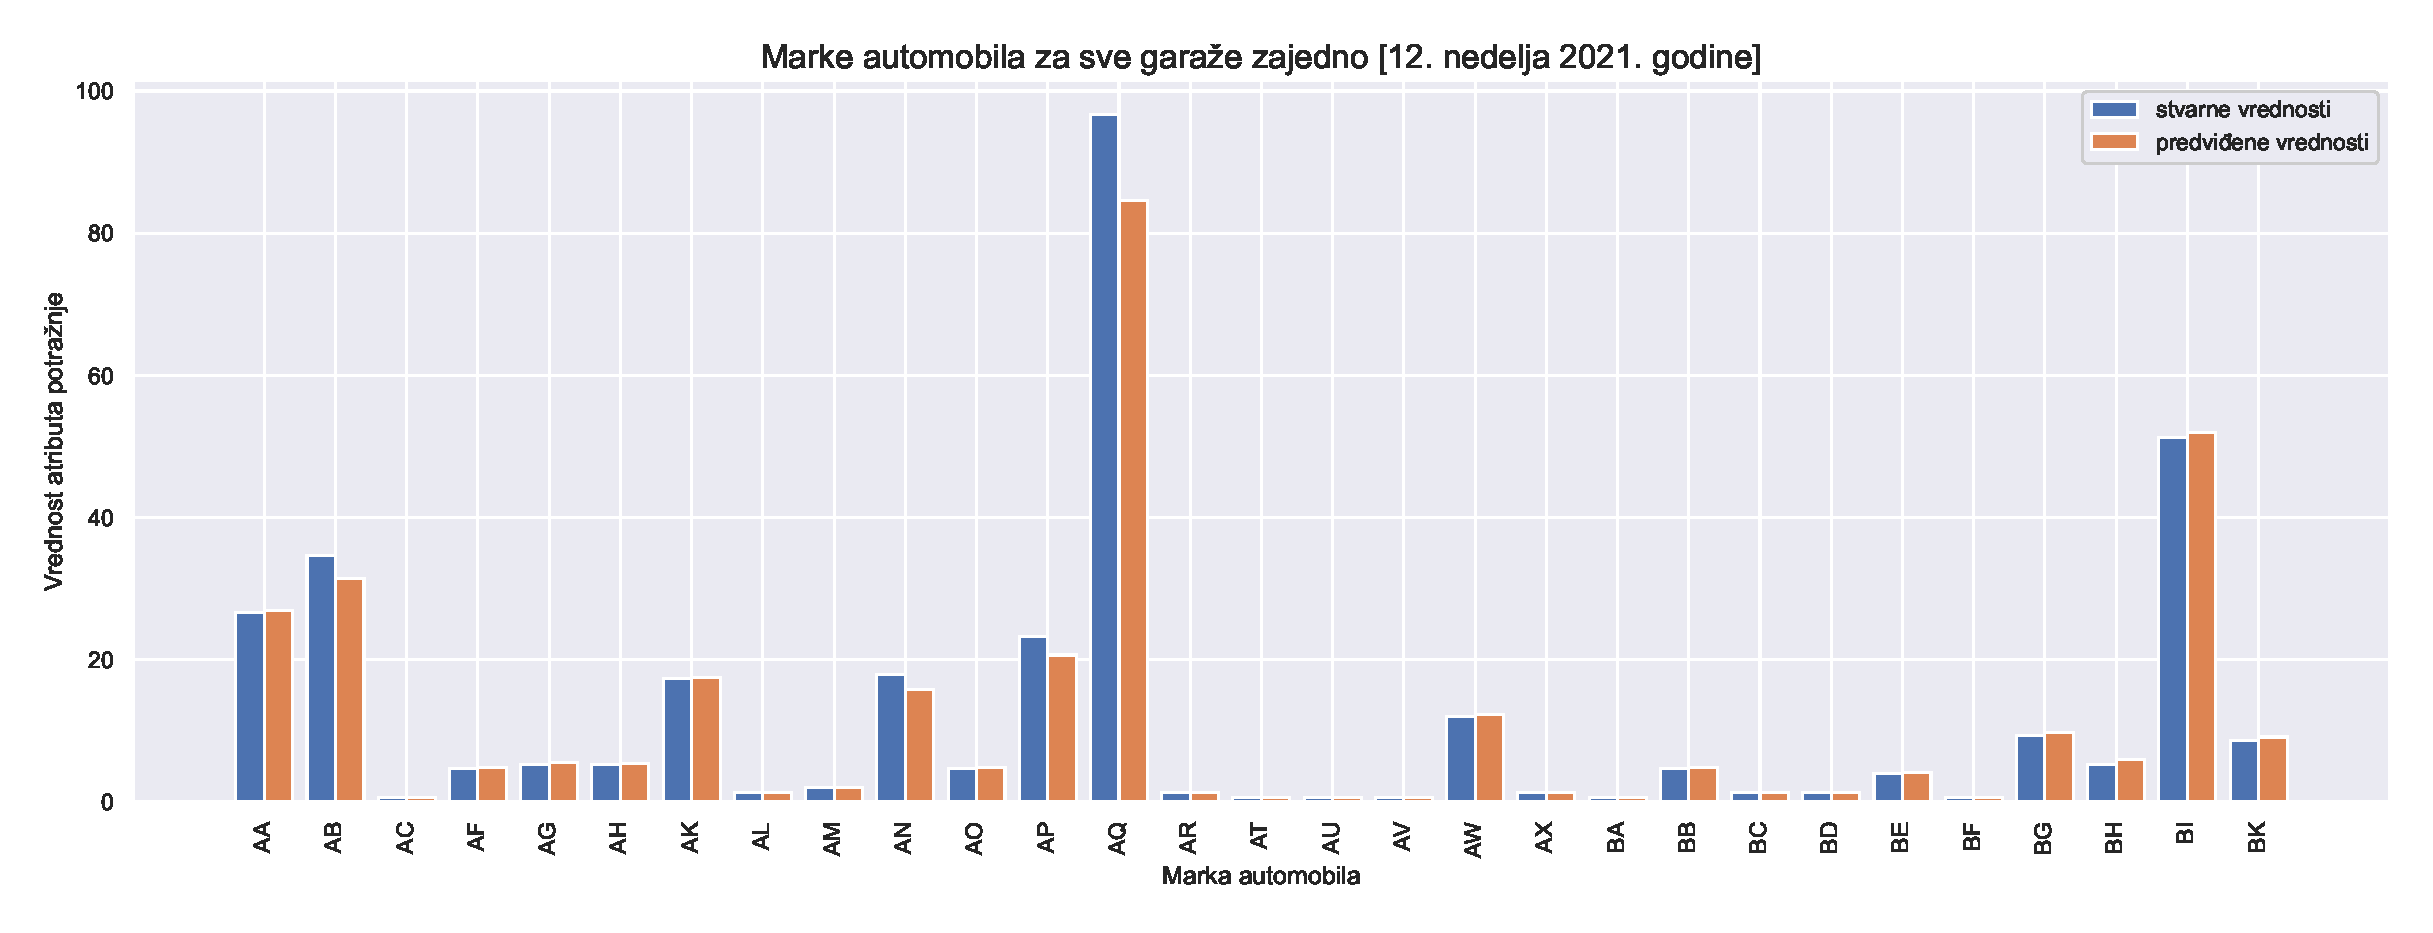
\includegraphics[width=1\textwidth]{./grafici/year_week_garage_make_train_on_all_available_202112.eps}
  \caption{Raspodela marki automobila za 12. nedelju 2021. godine.} 
  \label{fig: marke_nedelja}
\end{figure}

\begin{figure}[!ht]
  \centering
  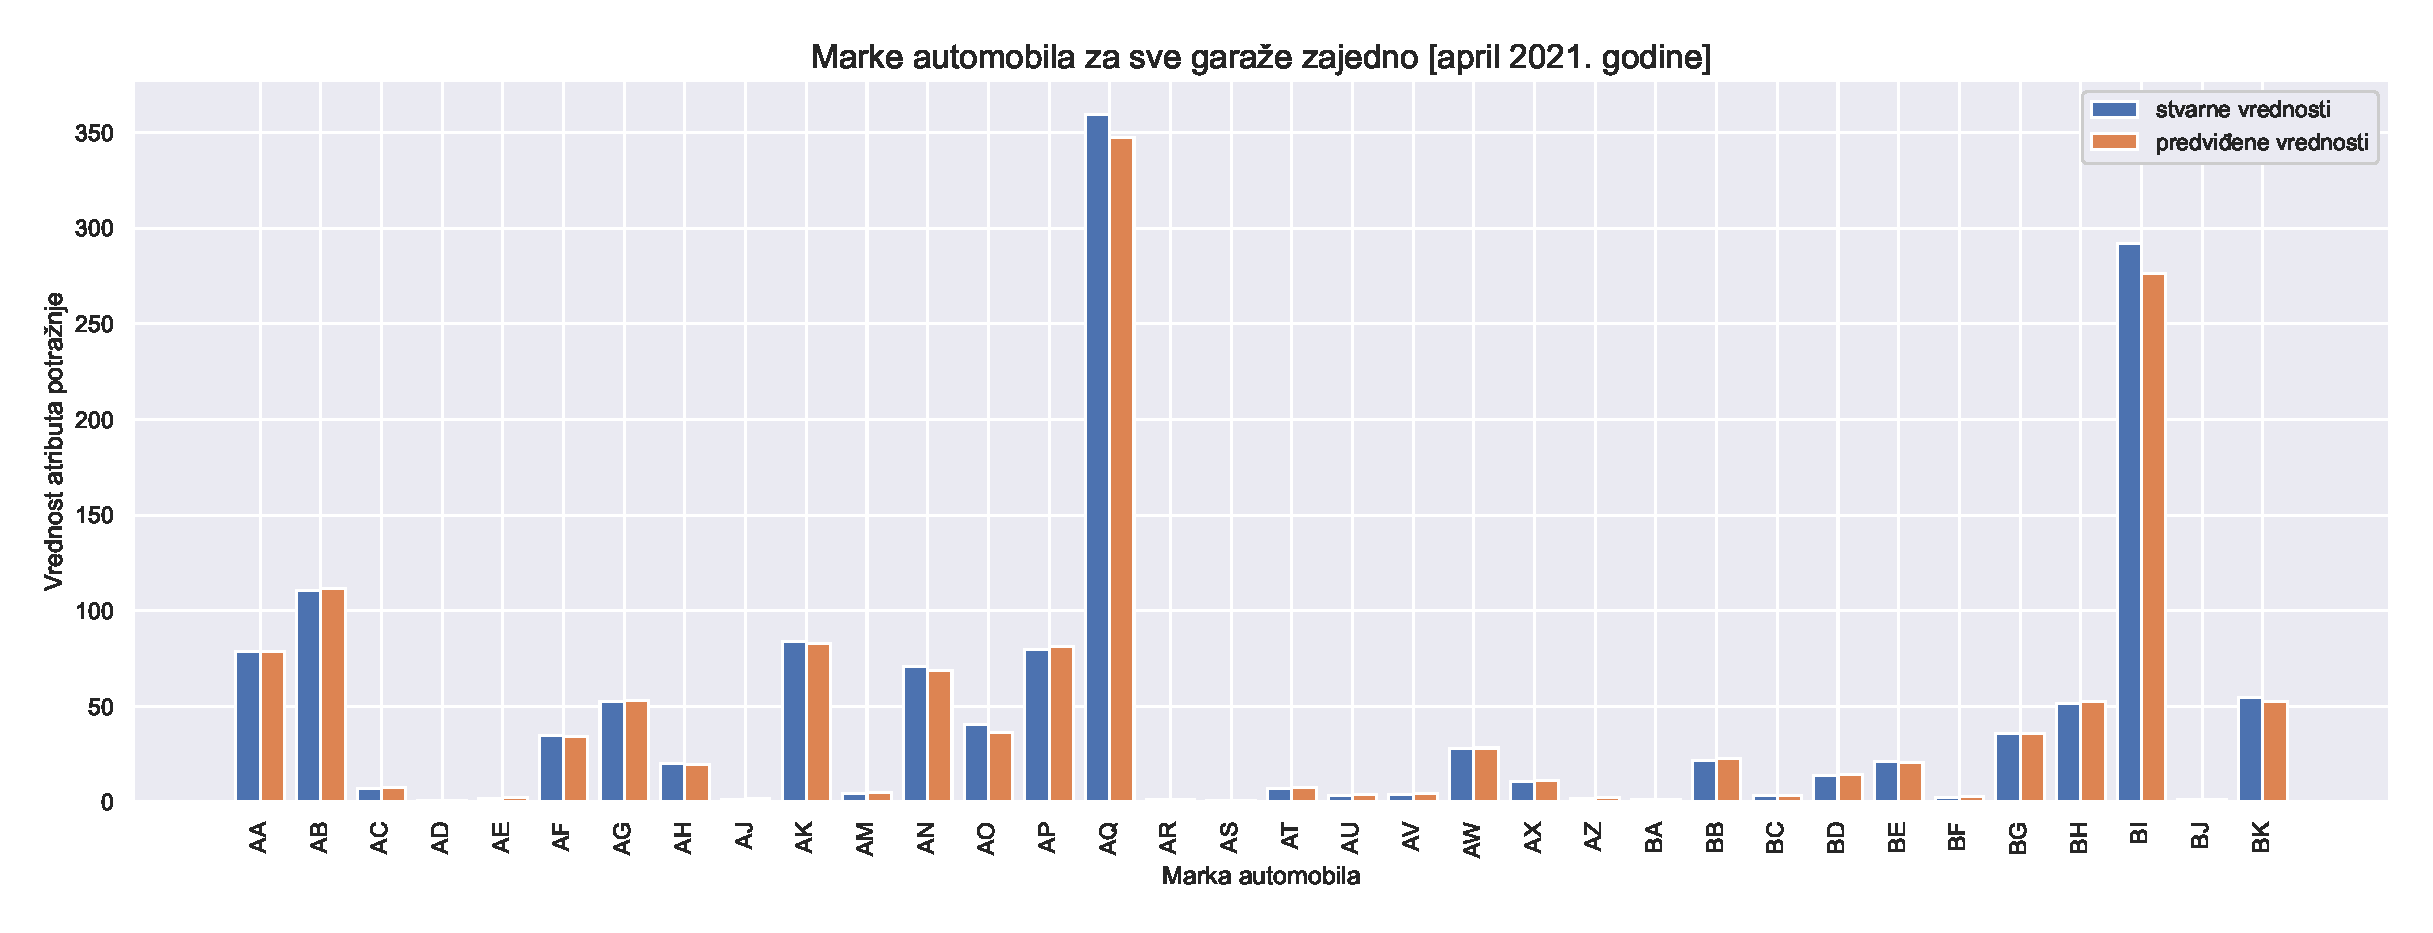
\includegraphics[width=1\textwidth]{./grafici/year_month_garage_make_train_on_all_available_202104.eps}
  \caption{Raspodela marki automobila za april mesec 2021. godine.}
  \label{fig: marke_mesec}
\end{figure}

\section{Diskusija rezultata}
% ------------------------------------------------------------------------------
Prethodne sekcije doprinele su da se bolje razumeju trenutno dostupni podaci. Otkriveno je da veliki broj automehaničarskih radnji spada u "manje" radnje, odnosno da mnoge od njih imaju veoma nisku vrednost ciljne promenljive \textit{demand\_value} koja je predviđana ili je uopšte nemaju za dosta vremenskih trenutaka. To znači da je za problem vremenskih serija agregacija podataka na neki način bila neophodna i da posmatranje vremenskih serija za svaku automehaničarsku radnju po automobilskim markama još uvek nema značajan broj podataka.

Takođe, potrebno je da se novi izvor podataka (booking portal) sa kog su podaci i prikupljeni, još više aktivira kako bi reprezentacija podataka bolje predstavljala radnje ili da se podaci obogate i svim drugim izvorima podataka koji postoje za sve automehaničarske radnje (što je problem na kom se radi).

Dobra strana istraživanja vremenskih serija i XGBoost metoda na način na koji je posmatran za dnevne i nedeljne podatke, je da se vrednosti prethodnih dana/nedelja mogu ubaciti kao novi veštački atribut u skup atributa za predviđanje metodama mašinskog učenja, jer se pokazalo da postoji neki smisao ubacivanja vrednosti lagova (vrednosti iz prošlosti) i da to može da doprinese modelu da uči. Broj vrednosti lagova bi mogao biti određen Arimom i njenim koeficijentima.

Prophet je pre svega ispitivan zbog ideje da ima podršku da uračuna efekte praznika na uticaj modela. Kroz istraživanje se pokazalo da je bolje ubaciti efekte praznika i da oni mogu da imaju značajne efekte na model. Pre svega je grafik vremenske serije na nedeljnom nivou otkrio značajne padove oko nekih datuma koji potencijalno nastaju zbog praznika.

Predstavljeno klasterovanjo automobilskih marki je davalo lošije rezultate, tako da je odbačena ideja klasterovanja automobila na predložen način. Potrebno je isprobati klasterovanje po nekom drugom kriterijumu, a možda i klasterovanje radnji treba uzeti u razmatranje, kako bi podaci ipak bili agregirani, ali ne suviše zbog manjka podataka. 

Uočen je i problem posmatranja problema kao sasvim regresionog problema kod XGBoost metode. Dolazak određene automobilske marke u neku automehaničarsku radionicu biva zabeležen i model se recimo obučava na takvim podacima, ali generalno regresioni problem neće da kaže da li je određena automobilska marka uopšte došla ili nije u automehaničarsku radnju. Dakle, potencijalno bi prvo trebalo uraditi binarnu klasifikaciju da je model došao ili nije došao i onda predviđati potražnju pomenute ciljne promenljive.

\chapter{Zaključak i pravci daljeg rada}
% ------------------------------------------------------------------------------
Kao što je pomenuto u uvodnom delu, problem predviđanja potražnje je široko zastupljen problem. U automobilskoj industriji precizno predviđanje može da dovede do optimizacije mnogih poslova, a samim tim i do uštede resursa, odnosno povećanja profita. Poslovi koji se mogu optimizovati u ovom konkretnom slučaju su naručivanja potrebne i dovoljne količine automobilskih delova, optimalnog distribuiranja tih delova do automehaničarskih radnji, pametno postavljanje popusta na popravke određenih automobilskih marki kako bi se povećali prihodi, a iskoristili neki zaostali delovi itd.

Ovaj rad je pokušao da načne novi problem koji je predstavljen od strane industrijskog sveta. Rad nad realnim podacima je kao i uvek dosta izazovan, posebno u slučaju kada podataka ima jako malo i u ovom slučaju gde je situacija da je izvor za podatke krenuo sa radom kao inovativna i nova ideja tek krajem 2019. godine. Nakon samog pokretanja desila se velika pandemija virusa i to je svakako uticalo da svi ovi dostupni podaci budu na neki način neobični. To će biti interesantno istraživati u godinama koje tek dolaze, sa povećanjem količine podataka. Takođe, kada se prikupe i podaci iz drugih izvora koji su vezani za sve automehaničarske radnje, mogao bi da se ispita uticaj booking portala na globalnu sliku rada kompanije. Istraživanje je pokazalo da modeli mogu dobro da se ponašaju na agregiranom nivou (recimo nivou cele države) ili na nivou predviđanja velikih automehaničarskih radnji za koje postoje dovoljne količine podataka. Za male radnje postoji veliki problem sa nepostojećim informacijama vezanim za marke automobila, tako da bi možda neki drugi problem (klasifikacija+regresija) mogao da pomogne. Takođe, bitno je napomenuti da ono što je prema podacima sa booking portala mala ili velika radnja, ne mora da bude realna slika. To može da bude samo usled dostupnih podataka ili usled toga što se neka velika radnja tek skoro priključila ozbiljnijem korišćenju ovog načina rezervisanja popravki, pa deluje kao da je mala po količini ciljne promenljive. To se može nadomestiti dobijanjem pristupa drugim izvorima podataka u ovoj kompaniji.

Istraživanje je otvorilo i neke nove ideje. Pre svega sledeći korak bi mogao biti obogaćivanje trenutnih podataka podacima koji su javno dostupni, a vezani za vremensku prognozu. Moguće je za svaki vremenski trenutak i na osnovu lokacija automehaničarskih radnji dodati atribut koji bi predstavljao svojstva vremenske prognoze, kako bi se uočilo da li zima/leto imaju uticaj na to kada ljudi popravljaju svoje automobile. Takođe, više informacija o samim korisnicima/garažama/automobilima bi doprinelo boljem klasterovanju podataka. Informacije o svakom automobilu koji je bio na popravci sadrže godinu proizvodnje, tako da se može gledati u pravcu da se obogaćivanje podataka vrši proširivanjem aproksimirane cene tog automobila i nekakve grupacije na osnovu tih informacija. Korišćenje Google Mapa umesto Open Street Mapa može doprineti preciznijem stanju, a možda i dobijanje javnih statističkih informacija o konkurentnim radnjama može da se uzme u obzir. Uzimanje više ličnih informacija korisnika ili više informacija o automobilima (pređena kilometraža, broj ukupnih vlasnika, broj oštećenja itd.) prilikom unosa rezervacije na booking portal, bi takođe moglo biti iskorišćeno u svrhe boljeg klasterovanja, a samim tim i predviđanja.

% ------------------------------------------------------------------------------
% Literatura
% ------------------------------------------------------------------------------
\literatura

% ==============================================================================
% Završni deo teze i prilozi
\backmatter
% ==============================================================================

% ------------------------------------------------------------------------------
% Biografija kandidata
\begin{biografija}
\shorthandon{"}%

  \textbf{Anđelka Milovanović} je rođena u Valjevu na datum koji predstavlja aproksimativnu vrednost broja $\pi$, dakle 22. jula 1996. godine. Išla je u Osnovnu školu "`Sestre Ilić" u Valjevu i u Muzičku školu "`Živorad Grbić", odsek za flautu. Nakon završene osnovne škole, kao najbolji đak svoje generacije, upisala je specijalizovano-matematičko odeljenje u Valjevskoj gimnaziji. Paralelno sa gimnazijom, pohađala je srednju muzičku školu za flautu nekoliko meseci, dok se nije javilo interesovanje za neke druge oblasti. 
  
  Tokom srednje škole bila je polaznica seminara astronomije u Istraživačkoj stanici Petnica sve četiri godine i vodila je astronomsku grupu u Društvu istraživača "`Vladimir Mandić-Manda" u Valjevu. Organizovala je aktivnosti poput akcija za posmatranje meteorskih rojeva i drugih nebeskih objekata, pomračenja Sunca i Meseca, Sata za našu planetu, zimskih i letnjih astronomskih škola za učenike osnovnih i srednjih škola, raznih naučno-popularnih predavanja i mnoge druge. Fokus tokom srednje škole joj je uglavnom bio na vaannastavnim aktivnostima, tako da je bila jedan od organizatora prvog Festivala nauke u gimnaziji, volontirala je na događajima Centra za promociju nauke i učestvovala na Astro-vikendu u Domu Omladine Beograda. 
  
  Najinteresantnija oblast u srednjoj školi joj je bilo programiranje, tako da odlučuje da upiše smer Informatike na Matematičkom fakultetu u Beogradu. Nakon 2. godine fakulteta dobija punu stipendiju Američke Vlade za jednosemestralnu studentsku razmenu "`Global UGRAD", na Univerzitetu na Floridi - Florida Gulf Coast University. Nakon godinu dana pauze na Matematičkom fakultetu, vraća se svojim studijama. Na početku 4. godine studija dobija besplatnu kartu od fakulteta za učešće na PyCon konferenciji u Beogradu, koja je dovodi do osvajanja 1. mesta na lokalnom i globalnom hakatonu (TADHack 2019) zajedno sa svoja dva drugara. Iste godine je provela 1. semestar u ulozi studenta demonstratora na kursu Računarske grafike, a 2. semestar u ulozi praktikanta u Microsoft Development Centru Srbije.    
  
  Nakon uspešno završenih osnovnih studija na Matematičkom fakultetu, Anđelka nastavlja obrazovanje i upisuje master studije na istom smeru, pokušavajući da otkrije koja oblast je najviše interesuje. Iste godine dobija diplomu Društva istraživača, kao potvrdu velikog zalaganja za popularizaciju nauke i samog društva tokom srednjoškolskog perioda. 
\shorthandoff{"}%
\end{biografija}
% ------------------------------------------------------------------------------

\end{document}
